% Options for packages loaded elsewhere
\PassOptionsToPackage{unicode}{hyperref}
\PassOptionsToPackage{hyphens}{url}
%
\documentclass[
]{article}
\usepackage{amsmath,amssymb}
\usepackage{lmodern}
\usepackage{iftex}
\ifPDFTeX
  \usepackage[T1]{fontenc}
  \usepackage[utf8]{inputenc}
  \usepackage{textcomp} % provide euro and other symbols
\else % if luatex or xetex
  \usepackage{unicode-math}
  \defaultfontfeatures{Scale=MatchLowercase}
  \defaultfontfeatures[\rmfamily]{Ligatures=TeX,Scale=1}
\fi
% Use upquote if available, for straight quotes in verbatim environments
\IfFileExists{upquote.sty}{\usepackage{upquote}}{}
\IfFileExists{microtype.sty}{% use microtype if available
  \usepackage[]{microtype}
  \UseMicrotypeSet[protrusion]{basicmath} % disable protrusion for tt fonts
}{}
\makeatletter
\@ifundefined{KOMAClassName}{% if non-KOMA class
  \IfFileExists{parskip.sty}{%
    \usepackage{parskip}
  }{% else
    \setlength{\parindent}{0pt}
    \setlength{\parskip}{6pt plus 2pt minus 1pt}}
}{% if KOMA class
  \KOMAoptions{parskip=half}}
\makeatother
\usepackage{xcolor}
\usepackage[margin=1in]{geometry}
\usepackage{color}
\usepackage{fancyvrb}
\newcommand{\VerbBar}{|}
\newcommand{\VERB}{\Verb[commandchars=\\\{\}]}
\DefineVerbatimEnvironment{Highlighting}{Verbatim}{commandchars=\\\{\}}
% Add ',fontsize=\small' for more characters per line
\usepackage{framed}
\definecolor{shadecolor}{RGB}{248,248,248}
\newenvironment{Shaded}{\begin{snugshade}}{\end{snugshade}}
\newcommand{\AlertTok}[1]{\textcolor[rgb]{0.94,0.16,0.16}{#1}}
\newcommand{\AnnotationTok}[1]{\textcolor[rgb]{0.56,0.35,0.01}{\textbf{\textit{#1}}}}
\newcommand{\AttributeTok}[1]{\textcolor[rgb]{0.77,0.63,0.00}{#1}}
\newcommand{\BaseNTok}[1]{\textcolor[rgb]{0.00,0.00,0.81}{#1}}
\newcommand{\BuiltInTok}[1]{#1}
\newcommand{\CharTok}[1]{\textcolor[rgb]{0.31,0.60,0.02}{#1}}
\newcommand{\CommentTok}[1]{\textcolor[rgb]{0.56,0.35,0.01}{\textit{#1}}}
\newcommand{\CommentVarTok}[1]{\textcolor[rgb]{0.56,0.35,0.01}{\textbf{\textit{#1}}}}
\newcommand{\ConstantTok}[1]{\textcolor[rgb]{0.00,0.00,0.00}{#1}}
\newcommand{\ControlFlowTok}[1]{\textcolor[rgb]{0.13,0.29,0.53}{\textbf{#1}}}
\newcommand{\DataTypeTok}[1]{\textcolor[rgb]{0.13,0.29,0.53}{#1}}
\newcommand{\DecValTok}[1]{\textcolor[rgb]{0.00,0.00,0.81}{#1}}
\newcommand{\DocumentationTok}[1]{\textcolor[rgb]{0.56,0.35,0.01}{\textbf{\textit{#1}}}}
\newcommand{\ErrorTok}[1]{\textcolor[rgb]{0.64,0.00,0.00}{\textbf{#1}}}
\newcommand{\ExtensionTok}[1]{#1}
\newcommand{\FloatTok}[1]{\textcolor[rgb]{0.00,0.00,0.81}{#1}}
\newcommand{\FunctionTok}[1]{\textcolor[rgb]{0.00,0.00,0.00}{#1}}
\newcommand{\ImportTok}[1]{#1}
\newcommand{\InformationTok}[1]{\textcolor[rgb]{0.56,0.35,0.01}{\textbf{\textit{#1}}}}
\newcommand{\KeywordTok}[1]{\textcolor[rgb]{0.13,0.29,0.53}{\textbf{#1}}}
\newcommand{\NormalTok}[1]{#1}
\newcommand{\OperatorTok}[1]{\textcolor[rgb]{0.81,0.36,0.00}{\textbf{#1}}}
\newcommand{\OtherTok}[1]{\textcolor[rgb]{0.56,0.35,0.01}{#1}}
\newcommand{\PreprocessorTok}[1]{\textcolor[rgb]{0.56,0.35,0.01}{\textit{#1}}}
\newcommand{\RegionMarkerTok}[1]{#1}
\newcommand{\SpecialCharTok}[1]{\textcolor[rgb]{0.00,0.00,0.00}{#1}}
\newcommand{\SpecialStringTok}[1]{\textcolor[rgb]{0.31,0.60,0.02}{#1}}
\newcommand{\StringTok}[1]{\textcolor[rgb]{0.31,0.60,0.02}{#1}}
\newcommand{\VariableTok}[1]{\textcolor[rgb]{0.00,0.00,0.00}{#1}}
\newcommand{\VerbatimStringTok}[1]{\textcolor[rgb]{0.31,0.60,0.02}{#1}}
\newcommand{\WarningTok}[1]{\textcolor[rgb]{0.56,0.35,0.01}{\textbf{\textit{#1}}}}
\usepackage{longtable,booktabs,array}
\usepackage{calc} % for calculating minipage widths
% Correct order of tables after \paragraph or \subparagraph
\usepackage{etoolbox}
\makeatletter
\patchcmd\longtable{\par}{\if@noskipsec\mbox{}\fi\par}{}{}
\makeatother
% Allow footnotes in longtable head/foot
\IfFileExists{footnotehyper.sty}{\usepackage{footnotehyper}}{\usepackage{footnote}}
\makesavenoteenv{longtable}
\usepackage{graphicx}
\makeatletter
\def\maxwidth{\ifdim\Gin@nat@width>\linewidth\linewidth\else\Gin@nat@width\fi}
\def\maxheight{\ifdim\Gin@nat@height>\textheight\textheight\else\Gin@nat@height\fi}
\makeatother
% Scale images if necessary, so that they will not overflow the page
% margins by default, and it is still possible to overwrite the defaults
% using explicit options in \includegraphics[width, height, ...]{}
\setkeys{Gin}{width=\maxwidth,height=\maxheight,keepaspectratio}
% Set default figure placement to htbp
\makeatletter
\def\fps@figure{htbp}
\makeatother
\setlength{\emergencystretch}{3em} % prevent overfull lines
\providecommand{\tightlist}{%
  \setlength{\itemsep}{0pt}\setlength{\parskip}{0pt}}
\setcounter{secnumdepth}{-\maxdimen} % remove section numbering
\newlength{\cslhangindent}
\setlength{\cslhangindent}{1.5em}
\newlength{\csllabelwidth}
\setlength{\csllabelwidth}{3em}
\newlength{\cslentryspacingunit} % times entry-spacing
\setlength{\cslentryspacingunit}{\parskip}
\newenvironment{CSLReferences}[2] % #1 hanging-ident, #2 entry spacing
 {% don't indent paragraphs
  \setlength{\parindent}{0pt}
  % turn on hanging indent if param 1 is 1
  \ifodd #1
  \let\oldpar\par
  \def\par{\hangindent=\cslhangindent\oldpar}
  \fi
  % set entry spacing
  \setlength{\parskip}{#2\cslentryspacingunit}
 }%
 {}
\usepackage{calc}
\newcommand{\CSLBlock}[1]{#1\hfill\break}
\newcommand{\CSLLeftMargin}[1]{\parbox[t]{\csllabelwidth}{#1}}
\newcommand{\CSLRightInline}[1]{\parbox[t]{\linewidth - \csllabelwidth}{#1}\break}
\newcommand{\CSLIndent}[1]{\hspace{\cslhangindent}#1}
\usepackage{float}
\ifLuaTeX
  \usepackage{selnolig}  % disable illegal ligatures
\fi
\IfFileExists{bookmark.sty}{\usepackage{bookmark}}{\usepackage{hyperref}}
\IfFileExists{xurl.sty}{\usepackage{xurl}}{} % add URL line breaks if available
\urlstyle{same} % disable monospaced font for URLs
\hypersetup{
  pdftitle={FishErIes Size and functional TYpe model (FEISTY) in R},
  pdfauthor={DDDD, BBBB, EEEE, and AAAA},
  hidelinks,
  pdfcreator={LaTeX via pandoc}}

\title{FishErIes Size and functional TYpe model (FEISTY) in R}
\author{DDDD, BBBB, EEEE, and AAAA}
\date{2024}

\begin{document}
\maketitle

\hypertarget{introduction}{%
\section{Introduction}\label{introduction}}

This vignette provides a comprehensive description of the model
equations, parameters, and numerical implementation used in the
FishErIes Size and functional TYpe (FEISTY) model system
(\protect\hyperlink{ref-petrik2019bottom}{Petrik et al. 2019};
\protect\hyperlink{ref-van2021emergent}{Denderen et al. 2021};
\protect\hyperlink{ref-thesubmittedpaper}{\textbf{thesubmittedpaper?}}).
This text is followed by several examples illustrating how to use the
model within R.

\hypertarget{the-feisty-model}{%
\section{The FEISTY model}\label{the-feisty-model}}

The FEISTY model framework is designed to be mechanistic, simple and
fast, generally applicable globally, and compatible with biogeochemical
model principles. It is based on ordinary differential equations and
careful accounting of mass balancing. The model structures fish around
functional types (aka. functional groups or guilds) based on traits
instead of representing specific species. This simplification, together
with the mechanistic basis, allows for projections into novel
environments, e.g., climate change projections.

The current FEISTY implementation includes four setups that define which
fish functional types are present and how they predate upon one another.
Two ``Basic'' setups contain three functional types: small and large
pelagic fish species and demersal species
(\protect\hyperlink{ref-petrik2019bottom}{Petrik et al. 2019}). Two
``Vertical'' setups augment the model with two additional functional
types, mesopelagic fish and midwater predators, and further automatize
the calculation of the interaction between the functional types based on
their vertical overlap (\protect\hyperlink{ref-van2021emergent}{Denderen
et al. 2021}). The Basic and Vertical setups with the suffix ``2''
modify the published setups with minor parameter and structural changes.
All setups are detailed below.

Regardless of the setup type the biomass dynamics follow the same set of
equations, which is detailed in the next section. The differences
between the setups lie in how the interactions between the types and
sizes are determined, which is detailed in the section ``Predation''.

\hypertarget{biomass-dynamics}{%
\subsection{Biomass dynamics}\label{biomass-dynamics}}

\hypertarget{fish-dynamics}{%
\subsubsection{Fish dynamics}\label{fish-dynamics}}

FEISTY is a size-based model where the biomass of each size class of a
functional type of fish (\(B_i\), gWW m\(^{-2}\)) \footnote{gWW: gram
  wet weight. From now on, we use ``g'' to represent ``gWW'' for
  simplicity.} changes over time (\(t\)) according to source and sink of
energy determined by consumption, growth, reproduction and mortality
(\protect\hyperlink{ref-deRoos2008}{De Roos et al. 2008}). The changes
in biomass are described by:

\begin{equation}
\dfrac{\mathrm{d}B_{i}}{\mathrm{d}t} =  J_{\mathrm{in},i}  + (\nu_{i} - \rho_i -\mu_i)B_i - J_{\mathrm{out},i},
\end{equation} where \(\nu_{i}\) is the rate of available energy for
growth and reproduction, \(\rho_i\) is the rate of reproduction, and
\(\mu_i\) is the total mortality rate. Fish growth leads to a flux out
of each size class, which enters the next size class. Since the largest
size-class of a functional type cannot grow to an even larger size, the
flux out of the last size-class is used for reproduction. The biomass
flux out of a size class \(i\) is: \begin{equation}
J_{\mathrm{out},i} = \gamma_i B_i,
\end{equation} where \(\gamma_i\) is the growth rate (year\(^{-1}\)).
The growth flux into a size class differs between the smallest
size-class of each functional type and the other sizes. These two parts
are: \begin{equation}
    J_{\mathrm{in},i} =
  \begin{cases}
\epsilon_r \left(  J_{\mathrm{out},n} + \sum\limits_i \rho_i B_i \right),      & \text{$ i=1 $} \\
     J_{\mathrm{out},i-1}, & \text{$ i > 1$} 
  \end{cases}
\end{equation} where \(\epsilon_r\) is the reproduction efficiency. The
flux into the smallest size class (\(i=1\)) is from the reproduction of
each size class of mature fish plus the biomass flux out of the size
class of a functional type (\(J_{\mathrm{out},n}\)). For all other size
classes (\(i > 1\)), the growth flux into the size class \(i\) is from
the growth of the previous neighboring size class (\(i-1\)).

\hypertarget{resource-dynamics}{%
\subsubsection{Resource dynamics}\label{resource-dynamics}}

FEISTY coupling with the biophysical forcing can be accomplished in
three ways: fully two-way (online), production-constrained one-way
(offline), and with resources as a semi-chemostat (offline). In case of
the latter, the resource \(i\) biomass dynamics change over time
according to a chemostat-like growth and consumption by fish predators.
The modelling of resources as a semi-chemostat is the default resource
dynamic mode in the four internal setups:

\begin{equation}
\dfrac{\mathrm{d}R_{i}}{\mathrm{d}t} =  r(K_i - R_i ) - \mu_{\mathrm{p},i} R_i,
\end{equation}

where \(R\) is the state variable of a resource, \(K\) is the carrying
capacity (g m\(^{-2}\)), and \(r\) is the growth rate which is a
constant value (1 year\(^{-1}\)). \(\mu_{\mathrm{p}}\) represents the
predation mortality on the resource. Lastly, FEISTY has an option to
model resource dynamics with the logistic growth equation:

\begin{equation}
\frac{\mathrm{d}R_i}{\mathrm{d}t}=r_i \cdot R_i \cdot (1-\frac{R_i}{K_i}) - \mu_{\mathrm{p},i} \cdot R_i,
\end{equation} which can be set in \texttt{paramAddResource()} function.

\hypertarget{physiological-rates}{%
\subsection{Physiological rates}\label{physiological-rates}}

There are three main biological rates based on the allometric scaling
relationship of individual body size: the mass-specific maximum
consumption rate \(C_{\mathrm{max},i}\) (year\(^{-1}\)), the
mass-specific clearance rate \(V_{i}\) (m\(^{2}\) g\(^{-1}\)
year\(^{-1}\)), and the mass-specific metabolic rate \(M_i\)
(year\(^{-1}\)): \begin{equation}
C_{\mathrm{max},i} = k_{\mathrm{T},i} \cdot a_{\mathrm{c}} \cdot m_{i}^{b_{\mathrm{c}}}  \label{eq:maxconsump}
\end{equation} \begin{equation}
V_{i} = k_{\mathrm{T},i} \cdot a_{\mathrm{e}} \cdot m_{i}^{b_{\mathrm{e}}}      \label{eq:clearance}
\end{equation} \begin{equation}
M_i = k_{\mathrm{TM},i} \cdot a_{\mathrm{m}} \cdot m_{i}^{b_{\mathrm{m}}}       \label{eq:metabolism}
\end{equation} Here \(k_{\mathrm{T},i}\) and \(k_{\mathrm{TM},i}\) are
scaling factors of temperature effects of each size class (see Section
\textbf{Temperature effects}). \(a_{\mathrm{c}}\), \(a_{\mathrm{e}}\),
and \(a_{\mathrm{m}}\) are factors for each biological rate;
\(b_{\mathrm{c}}\), \(b_{\mathrm{e}}\), and \(b_{\mathrm{m}}\) are
exponents. These biological rates determine the energy gained from
predation and costs due to basal metabolism (see Section \textbf{Energy
budget}).

In the code implementation, these basic biological rates of fish (set
against the reference temperature of 10\textdegree{}C) are assigned by
the \texttt{paramAddPhysiology()} function. The scaling of biological
rates with temperature is added subsequently (see Section
\textbf{Temperature effects}).

\hypertarget{energy-budget}{%
\subsection{Energy budget}\label{energy-budget}}

For a given individual size of fish \(m_i\), the mass-specific available
energy for growth or reproduction (rate) \(\nu_{i}\) is the result of
the mass-specific energy from assimilated food (rate) minus the
mass-specific metabolic rate: \begin{equation}
\nu_{i} = \epsilon_\alpha f_i C_{\mathrm{max},i} - M_i
\end{equation} where \(\epsilon_\alpha\) is the assimilation efficiency.
The mass-specific feeding level \(f_i\) (dimensionless) describes how
much food a predator can eat relative to the maximum consumption
capability, ranging from 0 to 1: \begin{equation}
f_{i} = \frac{E_{i}}{E_{i}+C_{\mathrm{max},i}}
\end{equation} Therefore, the mass-specific consumption rate
\(f_i C_{\mathrm{max},i}\) is based on type II functional response. The
feeding behavior of a predator is a consequence of encountering prey.
The mass-specific encounter rate (year\(^{-1}\)) \(E_{i}\) of a predator
\(i\) is: \begin{equation}
E_{i} = V_{i}  \sum_{j} \theta_{i,j} B_j,
\end{equation} where \(\theta_{i,j}\) denotes the feeding preference of
a predator \(i\) on a prey \(j\) (see Section \textbf{Predation}).
\(B_j\) represents the biomass of a prey \(j\) including zooplankton,
benthos, or fish. Therefore, the \(\sum_{j} \theta_{i,j} B_j\)
represents the biomass of all prey available to a predator.

\hypertarget{reproduction-and-growth}{%
\subsection{Reproduction and growth}\label{reproduction-and-growth}}

When the assimilated energy is positive after meeting the metabolic
demands, energy is available for fish growth and reproduction (when the
available energy is negative, there will be a biomass loss through
starvation). The reproductive rate (year\(^{-1}\)) of each size class of
fish is: \begin{equation}
\rho_i =
  \begin{cases}
 \psi_i \nu_i, & \text{$ \nu_i > 0 $}   \\
     0, & \text{$ \nu_i \leq 0 $} 
  \end{cases}
\end{equation} \(\psi_i\) is the maturity level (dimensionless) of fish
\(i\), describing the proportion of available energy (\(\nu_{i}\)) used
in the reproduction process. The maturity level can either be assigned
manually (setupBasic and setupVertical) or by a sigmoid function
(setupBasic2 and setupVertical2): \begin{equation}
\psi_i = \left(1+\left(\frac{m_{\mathrm{c},i}}{m_{\mathrm{mature}}}\right)^{-5} \right)^{-1}
\end{equation} where \(m_{\mathrm{mature}}\) is the half-maturation size
of a functional type, which means fish reach 50\% maturity level at
\(m_{\mathrm{mature}}\). \begin{equation}
m_{\mathrm{mature}} = \eta_{\mathrm{mature}} M
\end{equation} where \(\eta_{\mathrm{mature}}\) is the coefficient
determining the half-maturation size relative to the max size of a
functional type.

\(\kappa_{i}\) represents the fraction of the available energy
(\(\nu_{i}\)) invested in growth: \begin{equation}
\kappa_i = 1 - \psi_i
\end{equation}

The available energy for growth \(\kappa_i \nu_i\) gives a flux of
biomass out of the size-class \(i\) that depends on the ratio \(z\)
between the smallest and largest size of the size-class and total
mortality \(\mu_i\) (\protect\hyperlink{ref-deRoos2008}{De Roos et al.
2008}): \begin{equation}
 \gamma_i =
  \begin{cases}
\frac{ \kappa_i \nu_i - \mu_i }{1-(1/z)^{1-\mu_i/\kappa_i \nu_i}}, & \text{$ \nu_i > 0 $}   \\
     0, & \text{$ \nu_i \leq 0 $} 
  \end{cases}
\end{equation}

\(\mu_i\) includes a predation (\(\mu_{\mathrm{p},i}\)), background
(\(\mu_{\mathrm{b},i}\)), and fishing mortality rate
(\(\mu_{\mathrm{f},i}\)): \begin{equation}
\mu_i = \mu_{\mathrm{p},i}+\mu_{\mathrm{b},i}+\mu_{\mathrm{f},i}
\end{equation} All size classes of each functional type experience a
background mortality. The details of predation and fishing are described
in the sections below.

\hypertarget{predation}{%
\subsection{Predation}\label{predation}}

FEISTY specifies of how each size class (and zooplankton and benthic
prey resources) interact via predator-prey interactions in a feeding
preference matrix (also known as a food-web matrix). In this matrix,
each element \(\theta_{i,j}\) is a number between 0 and 1, which denotes
how much a fish class \(i\) preys on a prey class \(j\). The feeding
preference function is either based on size preference (see Section
\textbf{Size preference}) or derived from size preference coupling with
the vertical habitat of each functional group (see Section
\textbf{Vertical overlap}). For some combinations of predator and prey,
additional modifications are included to account for feeding
specializations (see Section \textbf{Modifications to the preference
matrix}).

Once the preference matrix is established, the predation mortality of a
prey \(j\) can be calculated: \begin{equation}
\mu_{\mathrm{p},j} = \sum_i  \frac{V_i \theta_{i,j}  B_i}{E_i+C_{\mathrm{max},i}} C_{\mathrm{max},i}
\end{equation}

\hypertarget{size-preference}{%
\subsubsection{Size preference}\label{size-preference}}

In the non-vertical setups (setupBasic and setupBasic2) \(\theta_{i,j}\)
refers to the feeding preference based on the size preference. In
setupVertical and setupVertical2, it is named \(\theta_{s,i,j}\) for
differentiation purposes. The value of \(\theta_{i,j}\) can be assigned
manually (setupBasic, see Table 2 in
(\protect\hyperlink{ref-petrik2019bottom}{Petrik et al. 2019})) or it
can be calculated using size-preference functions that are either based
on the log-normal distribution (setupBasic2 and setupVertical2):

\begin{equation}
 \theta_{i, j} =
  \begin{cases}
\exp\left( -\frac{\left(\log\left(\frac{m_{\mathrm{c},i}}{\beta \cdot m_{\mathrm{c},j}}\right)\right)^2}{(2 \cdot \sigma)^2} \right), & \text{$ m_{i} > m_{j} $}   \\
     0, & \text{$ m_{i} \leq m_{j} $} 
  \end{cases}
\label{eq:lognormalpreference}
\end{equation}

or the error function (setupVertical,
\protect\hyperlink{ref-van2021emergent}{Denderen et al. 2021}):
\begin{equation}
\theta_{i, j} = \frac{\sqrt{\frac{\pi}{2}} \cdot \sigma \cdot \left( \text{erf}\left(\frac{\log(m_{\mathrm{u},j}) - \log\left(\frac{m_{\mathrm{c},i}}{\beta}\right)}{\sqrt{2} \cdot \sigma}\right) - \text{erf}\left(\frac{\log(m_{\mathrm{l},j}) - \log\left(\frac{m_{\mathrm{c},i}}{\beta}\right)}{\sqrt{2} \cdot \sigma}\right) \right)}{\log(m_{\mathrm{u},j}) - \log(m_{\mathrm{l},j})}
\label{eq:errorpreference}
\end{equation} where \(\beta\) is preferred predator-prey mass ratio,
and \(\sigma\) is the size preference width for feeding. The
size-preference function selection and the values of \(\beta\) and
\(\sigma\) can be defined by the function \texttt{paramSizepref()}.

\hypertarget{vertical-overlap}{%
\subsubsection{Vertical overlap}\label{vertical-overlap}}

The vertical distribution in setupVertical and setupVertical2 is modeled
in a discretized water column: \begin{equation}
z_{\mathrm{\zeta}} =  0+\zeta, \hspace{1.5cm}  \zeta\in[0,z_{\mathrm{b}}]
\end{equation} where \(\zeta\) is each depth of a water column (integer
value), ranging from \(0\) (surface) to \(z_{\mathrm{bottom}}\) (sea
floor).

The vertical distribution of each size class and functional type \(i\)
is described as a unimodal distribution:

\begin{equation}
  \theta_{\mathrm{\zeta},\mathrm{x},i} = \frac{1}{\sqrt{2\pi\omega_i^2}} \cdot \exp\left(-\frac{(z_{\mathrm{\zeta}} - z_{\mathrm{loc},\mathrm{x},i})^2}{2\omega_i^2}\right)\\
  \label{eq:vertdist1}
\end{equation}

where \(\omega_i\) gives the vertical range of the vertical distribution
of each size class and functional type, \(\mathrm{x}\) is either day or
night, and \(z_{\mathrm{loc},\mathrm{x},i}\) is the defined water column
depth with the maximum biomass concentration. Some size classes in some
functional types have two depths with the maximum biomass concentration
\(z_{\mathrm{loc},\mathrm{x},i}\). Consequently, they need to be
calculated twice and the vertical distribution is the averaged value,
which shows a bimodal shape of the vertical distribution. The final
vertical distribution in either day or night at each depth of the water
column \(\mathrm{\zeta}\) is re-scaled so that the sum over the water
column is equal to one:

\begin{equation}
  \theta_{\mathrm{\zeta},\mathrm{x},i} = \frac{\theta_{\mathrm{\zeta},\mathrm{x},i}}{\sum\limits_{\mathrm{\zeta}} \theta_{\mathrm{\zeta},\mathrm{x},i}}
  \label{eq:vertdist2}
\end{equation}

The vertical range of the vertical distribution of each organism
\(\omega_i\) increases with body mass as larger individuals typically
have a wider habitat range: \begin{equation}
  \omega_i = \omega_0 + \tau \cdot \log_{10}\left(\frac{m_{\mathrm{c},i}}{m_{\mathrm{c},0}}\right)
\end{equation}

where \(\omega_0\) is the baseline range of the vertical distribution
and \(\tau\) is the range-increasing factor of vertical distribution.
\(m_{\mathrm{c},0}\) denotes the reference size to which all organisms
are scaled in the simulation (typically small mesozooplankton).

Vertical overlap between predator and prey is then estimated as the
lowest value between vertical distribution values of a specific predator
\(i\) and a prey \(j\) at depth \(\zeta\) at daytime or nighttime
\(\mathrm{x}\)
\(\min(\theta_{\mathrm{\zeta},\mathrm{x},i}, \theta_{\mathrm{\zeta},\mathrm{x},j})\).
The depth-integration gives the synthetic vertical overlap value of
predator \(i\) to a prey \(j\) at day or night
\(\theta_{\mathrm{v},\mathrm{x},i,j}\):

\begin{equation}
  \theta_{\mathrm{v},\mathrm{x},i,j} = \sum\limits_{\mathrm{\zeta}}\min(\theta_{\mathrm{\zeta},\mathrm{x},i},\theta_{\mathrm{\zeta},\mathrm{x},j})
\end{equation}

Ultimately, the total vertical overlap is the averaged value of the
synthetic day and night vertical overlap values:

\begin{equation}
  \theta_{\mathrm{v},i,j} = \frac{\theta_{\mathrm{v},\mathrm{day},i,j}+\theta_{\mathrm{v},\mathrm{night},i,j}}{2}
  \label{eq:vertover}
\end{equation}

This depth integrated vertical overlap value \(\theta_{\mathrm{v},i,j}\)
is combined with the size-based preference \(\theta_{\mathrm{s},i,j}\)
and used for the calculation of feeding preference \(\theta_{i,j}\):
\begin{equation}
\theta_{i,j} = \theta_{\mathrm{s},i,j} \cdot\theta_{\mathrm{v},i,j} 
\label{eq:verttheta}
\end{equation}

\hypertarget{vertical-habitats-of-resources-and-fish}{%
\subsubsection{Vertical habitats of resources and
fish}\label{vertical-habitats-of-resources-and-fish}}

Regardless of water conditions, Benthos are concentrated at the bottom
(\(z_{\mathrm{loc},\mathrm{day},i} = z_{\mathrm{loc},\mathrm{night},i} = z_{\mathrm{bottom}}\))
and to ensure they remain closely associated with the sea floor, their
vertical range is kept as the baseline value \(\omega_i=\omega_0\) (used
in Eq. \ref{eq:vertdist1}).

The vertical habitat strategy of fish depends on seafloor depth and
varies between fish functional types. Small and large pelagics and
demersal fish make up the fish community in shelf regions, i.e.~regions
\textless{} 250 meters in depth. In these regions, zooplankton prey,
small and large pelagics are distributed in the upper water column with
a maximum concentration at the surface of the water column
(\(z_{\mathrm{loc},\mathrm{day},i} = z_{\mathrm{loc},\mathrm{night},i} = 0\)).
Demersal fish change their vertical distribution throughout ontogeny
\footnote{small-, medium-, and large-size classes of fish are
  distinguished by comparison between the geometric mean mass value
  (\(m_{\mathrm{c},i}\)) and boundary mass value
  (\(m_{\mathrm{medium}}\) or \(m_{\mathrm{large}}\)). Small-size class:
  \(m_{\mathrm{c},i} < m_{\mathrm{medium}}\). Medium-size class:
  \(m_{\mathrm{medium}} \leq m_{\mathrm{c},i} \leq m_{\mathrm{large}}\).
  Large-size class: \(m_{\mathrm{c},i} > m_{\mathrm{large}}\). Default
  \(m_{\mathrm{medium}} = 0.5 \mathrm{g}\) and
  \(m_{\mathrm{large}} = 250 \mathrm{g}\) .}: small-size classes feed in
the upper water column
(\(z_{\mathrm{loc},\mathrm{day},i} = z_{\mathrm{loc},\mathrm{night},i} = 0\)),
medium-size classes feed at the bottom
(\(z_{\mathrm{loc},\mathrm{day},i} = z_{\mathrm{loc},\mathrm{night},i} = z_{\mathrm{bottom}}\)),
and large-size classes, if the water column is full of light
(\(z_{\mathrm{bottom}} \leq z_{\mathrm{photic}}\)), exhibit
cross-habitat feeding between the bottom and the surface waters all the
day with maximum concentrations at the surface and the bottom (two
\(z_{\mathrm{loc},\mathrm{x},i}\) for each day and night: 0 and
\(z_{\mathrm{bottom}}\)). If
(\(z_{\mathrm{bottom}} > z_{\mathrm{photic}}\)) large demersal fish stay
at surface waters during daytime
(\(z_{\mathrm{loc},\mathrm{day},i} = 0\)) and bottom at night
(\(z_{\mathrm{loc},\mathrm{night},i} = z_{\mathrm{bottom}}\)).

In slope and open ocean regions, some zooplankton resources and size
classes of specific fish functional types conduct diel vertical
migration to the depth \(z_{\mathrm{dvm}}\) (\(z_{\mathrm{dvmdem}}\) for
large demersal fish, described later), which is the representative depth
of maximum biomass concentration:

\begin{equation}
  z_{\mathrm{dvm}} =
  \begin{cases}
     z_{\mathrm{photc}} + 500, & \text{ $z_{\mathrm{bottom}} \geq z_{\mathrm{photic}} + 500$ } \\
     z_{\mathrm{bottom}}, & \text{ $ z_{\mathrm{photic}} + 500 > z_{\mathrm{bottom}} > z_{\mathrm{shelf}} $ } \\
     0, & \text{$ z_{\mathrm{bottom}} \leq z_{\mathrm{shelf}} $ }      
  \end{cases}
\label{eq:zdvm}
\end{equation}

The migrating part of the zooplankton community is at depth during the
day and at the surface at night, whereas the remaining zooplankton stay
at the surface waters the whole day
(\(z_{\mathrm{loc},\mathrm{day},i} = 0~and~z_{\mathrm{dvm}}\);
\(z_{\mathrm{loc},\mathrm{night},i} = 0\)). As a result, during the day,
zooplankton have a bimodal distribution with maximum concentration
depths at the surface and in the twilight zone.\\
Small pelagics are distributed in the upper water column with a maximum
concentration at the surface water
(\(z_{\mathrm{loc},\mathrm{day},i} = z_{\mathrm{loc},\mathrm{night},i} = 0\)).\\
Mesopelagic fish follow the day/night vertical movement of the migrating
zooplankton with a maximum concentration at similar depths
(\(z_{\mathrm{loc},\mathrm{day},i} = z_{\mathrm{dvm}}\);
\(z_{\mathrm{loc},\mathrm{night},i} = 0\)).\\
Large pelagics, perform differently throughout ontogeny. The small- and
medium-size classes are distributed in the upper water column with a
maximum concentration at the surface at day and night
(\(z_{\mathrm{loc},\mathrm{day},i} = z_{\mathrm{loc},\mathrm{night},i} = 0\)).
The large size-classes have a bimodal distribution during the day, where
half are distributed in the upper water column with a maximum
concentration at the surface (\(z_{\mathrm{loc},\mathrm{day},i} = 0\)),
and the other half have a maximum concentration in the midwater
(\(z_{\mathrm{loc},\mathrm{night},i} = z_{\mathrm{dvm}}\)). At night,
they are distributed in the upper water column
(\(z_{\mathrm{loc},\mathrm{night},i} = 0\)).\\
Small- and medium-size classes of midwater predators have the same
vertical distribution as mesopelagic fish
(\(z_{\mathrm{loc},\mathrm{day},i} = z_{\mathrm{dvm}}\);
\(z_{\mathrm{loc},\mathrm{night},i} = 0\)). Large midwater predators
have a maximum concentration in midwater
(\(z_{\mathrm{loc},\mathrm{day},i} = z_{\mathrm{loc},\mathrm{night},i} = z_{\mathrm{dvm}}\)).\\
Small demersals are distributed in the upper water column with a maximum
concentration at the surface both day and night
(\(z_{\mathrm{loc},\mathrm{day},i} = z_{\mathrm{loc},\mathrm{night},i} = 0\)).
Medium demersal fish are distributed near the bottom
(\(z_{\mathrm{loc},\mathrm{day},i} = z_{\mathrm{loc},\mathrm{night},i} = z_{\mathrm{bottom}}\)).
Large demersal fish have a vertical habitat strategy that differs from
the other groups. At night, large demersal fish are at the bottom
(\(z_{\mathrm{loc},\mathrm{night},i} = z_{\mathrm{bottom}}\)), while
during the day, the depth of maximum concentration
\(z_{\mathrm{dvmdem}}\) is:

\begin{equation}
  z_{\mathrm{dvmdem}} =
  \begin{cases}
     z_{\mathrm{dvm}}, & \text{ $ z_{\mathrm{bottom}} - z_{\mathrm{dvm}} < 1200 $ } \\
     z_{\mathrm{bottom}} - 1200, & \text{ $ 1200 \leq z_{\mathrm{bottom}} - z_{\mathrm{dvm}} <1500 $ } \\
     z_{\mathrm{bottom}}, & \text{ $ z_{\mathrm{bottom}} - z_{\mathrm{dvm}} \geq 1500 $ }      
  \end{cases}
\label{eq:zdvmdem}
\end{equation}

Table \ref{tab:vertloc} showed a summary of vertical habitats for
different resources and functional types.

\begin{table}[H]

\centering
\caption{ Representative depth of maximum biomass of each size class $z_{\mathrm{loc},\mathrm{x},i}$ at day and night. $z_{\mathrm{dvm}}$ and $z_{\mathrm{dvmdem}}$ can be found in Eq. \ref{eq:zdvm} and \ref{eq:zdvmdem}.}
\label{tab:vertloc}

\begin{tabular}{ l l l p{2cm} l l p{2cm}}
\hline
 & \multicolumn{3}{l}{Day} & \multicolumn{3}{l}{Night} \\
   \cline{2-7} 
Resources\\
\hline
Zooplankton$^a$ & \multicolumn{3}{l}{0 and $z_{\mathrm{dvm}}$} & \multicolumn{3}{l}{0} \\
Benthos & \multicolumn{3}{l}{$z_{\mathrm{bottom}}$} & \multicolumn{3}{l}{$z_{\mathrm{bottom}}$} \\
   \cline{2-7}
&\\   
Fish & Small & Medium & Large & Small & Medium & Large \\
\hline
Small pelagic fish & 0 & 0 & / & 0 & 0 & / \\
Mesopelagic fish & $z_{\mathrm{dvm}}$ & $z_{\mathrm{dvm}}$ & / & 0 & 0 & / \\
Large pelagic fish & 0 & 0 & 0 and $z_{\mathrm{dvm}}$ & 0 & 0 & 0 \\
Midwater predators & $z_{\mathrm{dvm}}$ & $z_{\mathrm{dvm}}$ & $z_{\mathrm{dvm}}$ & 0 & 0 & $z_{\mathrm{dvm}}$ \\
Demersal fish & 0 & $z_{\mathrm{bottom}}$ & $z_{\mathrm{dvmdem}}$$^b$ & 0 & $z_{\mathrm{bottom}}$ & $z_{\mathrm{bottom}}$$^b$ \\

\hline
\multicolumn{7}{l}{\footnotesize $^a$ Zooplankton include small and large mesozooplankton} \\
\multicolumn{7}{p{\dimexpr\linewidth-2\tabcolsep}}{\footnotesize $^b$ If the water column is shallower than the photic zone depth ($z_{\mathrm{bottom}} \leq z_{\mathrm{photic}}$), large demersal fish migrate over the water column (two  $z_{\mathrm{loc},\mathrm{x},i}$ for each day and night: $z_{\mathrm{dvmdem}}$ and $z_{\mathrm{bottom}}$). In such cases, $z_{\mathrm{dvmdem}}=0$.}

\end{tabular}
\end{table}

\hypertarget{modifications-to-the-preference-matrix}{%
\subsubsection{Modifications to the preference
matrix}\label{modifications-to-the-preference-matrix}}

\texttt{setupBasic2}

\begin{itemize}
\item
  The feeding preference from small pelagic and large pelagic fish to
  benthic resources and medium demersal fish are set to 0.
\item
  Large pelagic fish have a reduced feeding preference for medium-sized
  small pelagic fish (\(\theta_{\mathrm{A}} \cdot \theta_{i,j}\)).
\item
  The feeding preference from small demersal fish to benthic resources
  is set to 0.
\item
  Medium demersal fish only feed on benthos and themselves
  (cannibalism). Therefore, their feeding preference on zooplankton and
  all fish excluding themselves is corrected to 0.
\item
  Large demersal fish eat both pelagic and benthic organisms in shallow
  water (\(<~200\) m). They are less efficient at attacking pelagic prey
  and hence their feeding preference on small pelagic fish is
  down-regulated:
  \(\theta_{\mathrm{A}} \cdot \theta_{\mathrm{D}} \cdot \theta_{i,j}\);
  similarly for their feeding preference on large pelagic fish:
  \(\theta_{\mathrm{D}} \cdot \theta_{i,j}\). In deeper waters (\(>200\)
  m), large demersal fish only feed on benthos, medium demersals, and
  themselves.
\end{itemize}

\texttt{setupVertical\ and\ setupVertical2}

\begin{itemize}
\item
  Small and large pelagics are visual predators whose predation ability
  is better in light-rich waters during the day and worse in dark
  conditions such as night or the twilight zone. Therefore, according to
  habitats (Table \ref{tab:vertloc}), the vertical overlap is modified
  by multiplying it with a visual scaling factor
  \(\theta_{\mathrm{visual}}\): \begin{equation}
  \theta_{\mathrm{v},x,i,j} = \theta_{\mathrm{v},x,i,j} \cdot \theta_{\mathrm{visual}} .
  \end{equation} During daytime, the vertical overlap of all small and
  large pelagics on all preys in surface waters
  (\(\theta_{\mathrm{v},day,i,j}\)) is enhanced
  (\(\theta_{\mathrm{visual}}=1.5\)); the vertical overlap
  (\(\theta_{\mathrm{v},day,i,j}\)) of large size classes of large
  pelagics on the preys in the twilight zone (\(z_{\mathrm{dvm}}\))
  (mesopelagic fish and midwater predators) is reduced
  (\(\theta_{\mathrm{visual}}=0.5\)). At night, their vertical overlap
  on all preys (\(\theta_{\mathrm{v},night,i,j}\)) is decreased
  (\(\theta_{\mathrm{visual}}=0.5\)). Note this modification is done
  before Eq. \ref{eq:vertover}.
\item
  The feeding preference from all size-classes that are pelagic-living
  (small pelagics, mesopelagics, large pelagics, midwater predators and
  small size classes of demersal fish) to benthic resources are set to
  0. In addition, their feeding preference on medium demersal fish
  (benthic-living) is reduced
  (\(\theta_{i,j}=\theta_{i,j} \cdot 0.25\)).
\item
  The feeding preference of medium and large demersal fish to
  zooplankton resources are set to 0.
\item
  All large-size classes of pelagic-living functional fish groups (large
  pelagic fish, midwater predators, and demersal fish) have reduced
  feeding preference on medium-size small pelagic fish and medium-size
  mesopelagic fish
  (\(\theta_{i,j}=\theta_{i,j} \cdot \theta_{\mathrm{A}}\)).
\end{itemize}

\hypertarget{fishing-mortality}{%
\subsection{Fishing mortality}\label{fishing-mortality}}

The fishing mortality rate \(\mu_{\mathrm{f},i}\) of a particular size
class of fish \(i\) can be either determined by constant values or by a
fishing selectivity function
(\protect\hyperlink{ref-andersen2019fish}{Andersen 2019, chap. 5}):
\begin{equation}
\mu_{\mathrm{f},i}=\psi_{\mathrm{f},i}F_{\mathrm{max}}
\label{eq:fishing}
\end{equation} where \(F_{\mathrm{max}}\) is the baseline fishing
mortality rate (year\(^{-1}\)) of a functional type of fish.
\(\psi_{\mathrm{f},i}\) denotes a trawl-based fishing selectivity
following a sigmoid function: \begin{equation}
\psi_{\mathrm{f},i} = \left(1+\left(\frac{m_{\mathrm{c},i}}{m_{\mathrm{fishing}}}\right)^{-3} \right)^{-1}
\end{equation} where \(m_{\mathrm{fishing}}\) indicates the fish with
this size is under 50\% harvesting rate. \begin{equation}
m_{\mathrm{fishing}}=\eta_{\mathrm{F}} M
\end{equation} where \(\eta_{\mathrm{F}}\) controls the weight of fish
with a 50\% harvesting rate relative to the max weight of the functional
type. The fishing mortality rate can be assigned by the function
\texttt{setFishing()}.

\hypertarget{temperature-effects}{%
\subsection{Temperature effects}\label{temperature-effects}}

The temperature effects on the mass-specific maximum consumption rate
\(C_{\mathrm{max},i}\), the mass-specific clearance rate \(V_{i}\), and
the mass-specific metabolic rate \(M_i\) (Eq. \ref{eq:maxconsump},
\ref{eq:clearance}, \ref{eq:metabolism}) are based on the use of the
\(Q_{10}\) coefficient, which describes the exponential variation of
rates every 10\textdegree{}C.

The general equation for the temperature scaling factor \(k\) is:
\begin{equation}
k = Q_{10}^{\frac{T-T_{\mathrm{ref}}}{10}} \label{eq:Tscfac}
\end{equation} where \(T_{\mathrm{ref}}\) is the reference temperature
and \(T\) is the environment temperature. According to the different
functional types of fish and their sizes, fish habitats change. For fish
staying in the pelagic zone, \(T=T_{\mathrm{p}}\), which reflects the
average temperature in the top 100m of the water column. For fish in the
benthic zone, \(T=T_{\mathrm{b}}\), which reflects the temperature near
the bottom. Through introducing different \(Q_{10}\) coefficients (Table
\ref{tab:defaultparam}), various temperature scaling factors \(k\) can
be obtained. \(k_{\mathrm{T}}\) is the temperature scaling factor for
\(C_{\mathrm{max},i}\), and \(V_{i}\); \(k_{\mathrm{TM}}\) is the
temperature scaling factor for \(M_i\).

\textbf{setupBasic and setupBasic2}

In \texttt{setupBasic} and \texttt{setupBasic2}, there are three
functional types of fish: small pelagic fish, large pelagic fish, and
demersal fish. Small pelagics and large pelagics are always in the
pelagic water, so the \(T_{\mathrm{p}}\) is consistently applied.
Demersal fish habitats change according to size. Small demersal fish are
in a pelagic status (\(T_{\mathrm{p}}\)). Medium demersals live at the
bottom (\(T_{\mathrm{b}}\)). Large demersals also stay in the bottom if
the water is deep (\(>~200\) m). However, in shallow water (\(<~200\)
m), large demersals are assumed to spend a fraction of time \(\lambda\)
in the pelagic zone and the rest of time \(1-\lambda\) at the bottom
according to the abundance of prey in these two zones: \begin{equation}
\lambda = \frac{B_{\mathrm{pelprey}}}{B_{\mathrm{allprey}}}
\end{equation} where \(B_{\mathrm{pelprey}}\) denotes the total biomass
of pelagic prey for large demersal fish, \(B_{\mathrm{allprey}}\) is the
total biomass of all prey for large demersal fish. A simple case can be
found in Eq. 15 in (\protect\hyperlink{ref-petrik2019bottom}{Petrik et
al. 2019}).\\
Therefore, the temperature for large demersals is defined based on their
time spent in the pelagic zone and benthic zone, which is called
effective temperature:

\begin{equation} 
T_{\mathrm{e}} = T_{\mathrm{p}} \cdot \lambda + T_{\mathrm{b}} \cdot (1 - \lambda)
\end{equation}

In code implementation, temperature effects on biological rates are done
by the function \texttt{paramTeffect()}. Note this function only works
on non-vertical distribution setups, i.e., \texttt{setupBasic} and
\texttt{setupBasic2}. \(T_{\mathrm{e}}\) is updated each time step
during the time integration, along with the temperature-dependent
biological rates of large demersals, which are handled by the function
\texttt{updateET()}. The function \texttt{updateET()} is called every
time step in \texttt{derivativesFEISTYR()}. The effective temperature
scheme is forced turned on in \texttt{setupBasic()}
(\protect\hyperlink{ref-petrik2019bottom}{Petrik et al. 2019}); it is an
option in \texttt{setupBasic2()}.

\textbf{setupVertical}

In setupVertical, fish have a vertical distribution. Temperature effects
on physiological rates of each size class are based on where fish stay
in a water column (environmental temperature). Therefore the total
vertical distribution data needs to be calculated initially:

\begin{equation}
  \theta_{\mathrm{\zeta},i} = \frac{\theta_{\mathrm{\zeta},\mathrm{day},i}+\theta_{\mathrm{\zeta},\mathrm{night},i}}{2}
\end{equation}

Then the temperature scaling factor of each size class in a discretized
water column can be obtained according to their vertical distribution:

\begin{equation}
k_{\mathrm{\zeta},i} = \theta_{\mathrm{\zeta},i} \cdot Q_{10}^{\frac{T_{\mathrm{\zeta}}-T_{\mathrm{ref}}}{10}}
\end{equation}

where the water column temperature profile ranging from the surface (0
m) to the bottom, which can be obtained from observational data products
or earth system model outputs. Finally, the scaling factor is integrated
over the vertical distribution.

\begin{equation}
k_{i} = \sum\limits_{\mathrm{\zeta}} k_{\mathrm{\zeta},i}
\end{equation}

\(k_{i}\) can be used in temperature effects on physiological rates Eq.
\ref{eq:maxconsump}, \ref{eq:clearance}, \ref{eq:metabolism}. The
implementation is hard-coded, and embedded in the function
\texttt{setupVertical()}.

\textbf{setupVertical2}

To simplify the temperature input, three temperature inputs
(\(T_{\mathrm{p}}\), \(T_{\mathrm{m}}\), \(T_{\mathrm{b}}\)) are
required rather than the water column temperature profile in
setupVertical2. \(T_{\mathrm{m}}\) represents the averaged mid-water
temperature (500 - up to 1500 m). If \(T_{\mathrm{m}}\) is not provided,
\(T_{\mathrm{m}} = T_{\mathrm{b}}\) The effective temperature of
different size classes of each functional type are the averaged values
of temperatures of their approximate vertical positions of day
(\(T_{\mathrm{day}}\)) and night (\(T_{\mathrm{night}}\)).
\begin{equation}
T_{\mathrm{e}} = \frac{T_{\mathrm{day}}+T_{\mathrm{night}}}{2}
\end{equation}

Note this \(T_{\mathrm{e}}\) is different from the one in setupBasic and
setupBasic2. The \(T_{\mathrm{e}}\) is taken into Eq. \ref{eq:Tscfac} as
\(T\), and updates the temperature-dependent physiological rates (Eq.
\ref{eq:maxconsump}, \ref{eq:clearance}, \ref{eq:metabolism}). The
implementation is hard-coded in the function \texttt{setupVertical2()}.

The temperatures associated with each size class and functional type
follow the vertical distributions:

\begin{itemize}
\item
  Small pelagics always stay in the surface pelagic waters
  (\(T_{\mathrm{day}}=T_{\mathrm{night}}=T_{\mathrm{p}}\)).
\item
  Mesopelagics at night stay in the surface pelagic waters
  (\(T_{\mathrm{night}}=T_{\mathrm{p}}\)), whereas their vertical
  distribution varies with depth and photic conditions during the day:
\end{itemize}

\begin{equation}
 T_{\mathrm{day}} =
  \begin{cases}
     T_{\mathrm{m}}, & \text{$ z_{\mathrm{dvm}} \neq z_{\mathrm{bottom}} $ and $ z_{\mathrm{dvm}} \neq 0 $ } \\
     T_{\mathrm{b}}, & \text{$ z_{\mathrm{dvm}} = z_{\mathrm{bottom}} $} \\
     T_{\mathrm{p}}, & \text{$ z_{\mathrm{dvm}} = 0 $}      
  \end{cases}
\label{eq:xxxxxxxx}
\end{equation}

\begin{itemize}
\tightlist
\item
  The small and medium-sized classes of large pelagics are in the
  surface pelagic waters both day and night
  (\(T_{\mathrm{day}}=T_{\mathrm{night}}=T_{\mathrm{p}}\)). The
  large-sized classes of large pelagic fish are in the surface pelagic
  waters at night (\(T_{\mathrm{night}}=T_{\mathrm{p}}\)) and they are
  split into two groups during the day: half of them are always in the
  surface pelagic zone, and the habitat of the other half depends on the
  water column conditions. Their daytime temperature is the average of
  these two environmental temperatures:
\end{itemize}

\begin{equation}
 T_{\mathrm{day}} =
  \begin{cases}
     \frac{T_{\mathrm{m}}+T_{\mathrm{p}}}{2}, & \text{$ z_{\mathrm{dvm}} \neq z_{\mathrm{bottom}} $ and $ z_{\mathrm{dvm}} \neq 0 $ } \\
     \frac{T_{\mathrm{b}}+T_{\mathrm{p}}}{2}, & \text{$ z_{\mathrm{dvm}} = z_{\mathrm{bottom}} $} \\
     T_{\mathrm{p}}, & \text{$ z_{\mathrm{dvm}} = 0 $}      
  \end{cases}
\label{eq:xxxxxxx}
\end{equation}

\begin{itemize}
\item
  Midwater predators at daytime stay at the dvm depth, bottom, or
  surface pelagic zone, depending on the water column depth and photic
  conditions: \begin{equation}
   T_{\mathrm{day}} =
  \begin{cases}
     T_{\mathrm{m}}, & \text{$ z_{\mathrm{dvm}} \neq z_{\mathrm{bottom}} $ and $ z_{\mathrm{dvm}} \neq 0 $ } \\
     T_{\mathrm{b}}, & \text{$ z_{\mathrm{dvm}} = z_{\mathrm{bottom}} $} \\
     T_{\mathrm{p}}, & \text{$ z_{\mathrm{dvm}} = 0 $} 
  \end{cases}
  \label{eq:xxxxxxx2}
  \end{equation} At nighttime, small and medium midwater predators are
  in the surface pelagic waters (\(T_{\mathrm{night}}=T_{\mathrm{p}}\)),
  whereas the habitat of large midwater predators varies with water
  column conditions: \begin{equation}
   T_{\mathrm{night}} =
  \begin{cases}
     T_{\mathrm{m}}, & \text{$ z_{\mathrm{dvm}} \neq z_{\mathrm{bottom}} $ and $ z_{\mathrm{dvm}} \neq 0 $ } \\
     T_{\mathrm{b}}, & \text{$ z_{\mathrm{dvm}} = z_{\mathrm{bottom}} $} \\
     T_{\mathrm{p}}, & \text{$ z_{\mathrm{dvm}} = 0 $}  
  \end{cases}
  \label{eq:xxxxxx}
  \end{equation}
\item
  Small demersals are pelagic-living
  (\(T_{\mathrm{day}}=T_{\mathrm{night}}=T_{\mathrm{p}}\)); medium
  demersals are benthic-living
  (\(T_{\mathrm{day}}=T_{\mathrm{night}}=T_{\mathrm{b}}\)). Large
  demersal fish habitats vary according to the water column conditions.
\end{itemize}

\begin{equation}
 T_{\mathrm{day}} =
  \begin{cases}
     T_{\mathrm{m}}, & \text{$ (z_{\mathrm{bottom}} - z_{\mathrm{dvm}}) < 1500 $ and $ z_{\mathrm{bottom}} \geq z_{\mathrm{photic}} $} \\
     T_{\mathrm{b}}, & \text{$ (z_{\mathrm{bottom}} - z_{\mathrm{dvm}}) \geq 1500 $ } \\
     \frac{T_{\mathrm{b}}+T_{\mathrm{p}}}{2}, & \text{$ z_{\mathrm{bottom}} < z_{\mathrm{photic}} $} 
  \end{cases}
\label{eq:xxxxxx2}
\end{equation}

\begin{equation}
 T_{\mathrm{night}} =
  \begin{cases}
     T_{\mathrm{b}}, & \text{$ z_{\mathrm{bottom}} \geq z_{\mathrm{photic}} $}  \\
     \frac{T_{\mathrm{b}}+T_{\mathrm{p}}}{2}, & \text{$ z_{\mathrm{bottom}} < z_{\mathrm{photic}} $} 
  \end{cases}
\label{eq:xxxxxx3}
\end{equation}

\hypertarget{setup-of-the-size-spectrum-grid}{%
\subsection{Setup of the size spectrum
grid}\label{setup-of-the-size-spectrum-grid}}

The fish size span of a functional type is logarithmically discretized
into \(n\) continuous size bins. Each size bin shares the same ratio
\(z\) between the upper boundary size and lower boundary size:
\begin{equation}
z = \exp \left( \frac{\ln (M) - \ln (M_{0})}{n} \right)
\end{equation} where \(M_{0}\) and \(M\) are the smallest and largest
fish in a functional type (boundary size). There are \(n+1\) boundaries
of \(n\) size bins (\(m_{\mathrm{b},i}\)), including all lower boundary
sizes (\(m_{\mathrm{l},i}\)) and upper boundary sizes
(\(m_{\mathrm{u},i}\)). \begin{equation}
m_{\mathrm{b},i} =  \exp( \ln(M_{0}) + (i-1) \ln(z)), \hspace{1.5cm}  i\in[1,n+1]
\end{equation} \begin{equation}
m_{\mathrm{l},i} =  m_{\mathrm{b},i}, \hspace{5.5cm}  i\in[1,n]
\end{equation} \begin{equation}
m_{\mathrm{u},i} =  m_{\mathrm{b},i+1}, \hspace{5.1cm}  i\in[1,n]
\end{equation} The geometric mean size of each size class \(m_{i}\) is:
\begin{equation}
m_{i} =  \exp ( \ln(m_{\mathrm{l},i}) + 0.5(\ln(z)) ), \hspace{2.2cm}  i\in[1,n]
\end{equation} which can be comprehensively used for calculations, for
instance, physiological rates and size-based feeding preference.\\
The size spectrum generation is done by calling the function
\texttt{paramAddGroup()}. Also, see the source code of
\texttt{makeGrid()}.

\newpage

\hypertarget{default-parameters}{%
\section{Default parameters}\label{default-parameters}}

\begin{table}[htbp]

\centering
\caption{Main parameters of FEISTY}
\label{tab:defaultparam}

\begin{tabular}{lp{8cm}lp{1cm}lp{1cm}lp{1cm}lp{1cm}l}
\hline
Symbol & Description & \multicolumn{4}{c}{Value$^a$} & Unit \\
                         \cline{3-6}
       &             & \multicolumn{1}{c}{B1} & \multicolumn{1}{c}{B2} & \multicolumn{1}{c}{V1} & \multicolumn{1}{c}{V2} & \\
\hline
$a_\mathrm{c}$ & Intercept for mass-specific maximum consumption rate & \multicolumn{4}{c}{20} & g$^{-b_{\mathrm{c}}}$yr$^{-1}$ \\
$b_\mathrm{c}$ & Exponent for mass-specific maximum consumption rate & \multicolumn{4}{c}{-0.25} & / \\
$a_\mathrm{e}$ & Intercept for mass-specific clearance rate & \multicolumn{4}{c}{70} & m$^2$g$^{-b_{\mathrm{e}}-1}$yr$^{-1}$ \\
$b_\mathrm{e}$ & Exponent for mass-specific clearance rate & \multicolumn{4}{c}{-0.2} & / \\
$a_\mathrm{m}$ & Intercept for mass-specific metabolism rate & \multicolumn{4}{c}{0.2*$a_{\mathrm{c}}$} & g$^{-b_{\mathrm{m}}}$yr$^{-1}$ \\
$b_\mathrm{m}$ & Exponent for mass-specific metabolism rate & \multicolumn{4}{c}{-0.175} & / \\
$\epsilon_{\mathrm{\alpha}}$ & Assimilation efficiency & \multicolumn{4}{c}{0.7} & / \\
$\epsilon_{\mathrm{r}}$ & Reproduction efficiency & \multicolumn{4}{c}{0.01} & / \\
$\mu_\mathrm{b}$ & Background mortality & \multicolumn{4}{c}{0.1} & yr$^{-1}$ \\
$F_{\mathrm{max}}$ & Maximum fishing mortality rate & \multicolumn{4}{c}{0$^b$} & yr$^{-1}$ \\
$\eta_{\mathrm{mature}}$ & half-maturation size coefficient & /$^c$ & \multicolumn{3}{c}{0.25} & / \\
$\eta_{\mathrm{fishing}}$ & half-harvesting size coefficient & /$^d$ & \multicolumn{3}{c}{0.05} & / \\
$\theta_\mathrm{A}$ & Large fish preference on small pelagic fish$^e$ & \multicolumn{4}{c}{0.5} & / \\
$\theta_\mathrm{D}$ & Large demersal fish preference on pelagic prey & \multicolumn{2}{c}{0.75} & / & / & / \\
$\omega_0$ & baseline range of the vertical distribution & \multicolumn{2}{c}{/} & \multicolumn{2}{c}{10} & / \\
$\tau$ & range-increasing factor of vertical distribution & \multicolumn{2}{c}{/} & \multicolumn{2}{c}{10} & / \\
$T_{\mathrm{ref}}$ & reference temperature & \multicolumn{4}{c}{10} & \textdegree{}C \\
$Q_{\mathrm{10}}$ & Rate of change for every 10\textdegree{}C increase for clearance rate and maximum consumption & \multicolumn{4}{c}{1.88} & / \\
$Q_{\mathrm{10m}}$ & Rate of change for every 10\textdegree{}C increase for metabolism & \multicolumn{2}{c}{2.35} & \multicolumn{2}{c}{1.88} & / \\
$\beta$ & Preferred predator:prey mass ratio & / & \multicolumn{3}{c}{400} & / \\
$\sigma$ & Width of size preference for feeding & / & \multicolumn{3}{c}{1.3} & / \\
$z_{\mathrm{shelf}}$ & Continental shelf depth & / & / & \multicolumn{2}{c}{250} & m \\
$z_{\mathrm{photic}}$ & Photic zone depth & / & / & \multicolumn{2}{c}{150} & m \\
$m_{\mathrm{medium}}$ & boundary size of small/medium fish class & \multicolumn{4}{c}{0.5} & g \\
$m_{\mathrm{large}}$ & boundary size of medium/large fish class  & \multicolumn{4}{c}{250} & g \\

\hline
\multicolumn{7}{l}{\footnotesize $^a$ B1: setupBasic1, B2: setupBasic2, V1: setupVertcal1, V2: setupVertcal2.} \\
\multicolumn{7}{p{\dimexpr\linewidth-2\tabcolsep}}{\footnotesize $^b$ In B1, the fishing mortality can also be assigned manually [@petrik2019bottom] (Eq. \ref{eq:fishing} does not apply). $\mu_{f,i}$ are constant values: Small fish 0 yr$^{-1}$, Medium fish 0.03 yr$^{-1}$, Large fish 0.3 yr$^{-1}$.}\\
\multicolumn{7}{p{\dimexpr\linewidth-2\tabcolsep}}{\footnotesize $^c$ Maturity level $\psi_i$ is assigned manually in default B1. Only the last stage of each functional type has a value of 0.5 others are 0.} \\
\multicolumn{7}{l}{\footnotesize $^d$ Fishing  mortality $\mu_{f,i}$ is 0 in default B1.} \\
\multicolumn{7}{p{\dimexpr\linewidth-2\tabcolsep}}{\footnotesize $^e$ In B1, $\theta_{\mathrm{A}}$ only poses on medium-sized classes of small pelagic fish (the second size class).
                                      In B2, $\theta_{\mathrm{A}}$ works on all small pelagic fish. 
                                      In V1 and V2, $\theta_{\mathrm{A}}$ works on medium-sized classes of small pelagic and mesopelagic fish.} \\

\end{tabular}
\end{table}

\hypertarget{demonstration}{%
\section{Demonstration}\label{demonstration}}

FESITY includes four setups which each specifies the available
functional groups and their parameters:

\begin{itemize}
\tightlist
\item
  setupBasic creates a basic three-functional type setup as described in
  (\protect\hyperlink{ref-petrik2019bottom}{Petrik et al. 2019}).
\item
  setupBasic2 creates the same three-functional type setup as
  setupBasic(), but it allows more size numbers in each functional type,
  size-based maturity, generalized size-based feeding preference, and
  size-based fishing mortality.
\item
  setupVertical makes a basic five-functional type setup that includes
  vertical distribution of resources and fish
  (\protect\hyperlink{ref-van2021emergent}{Denderen et al. 2021}).
\item
  setupVertical2 is the same as setupVertical but different it allows
  more size numbers in each functional type, size-based maturity,
  generalized size-based feeding preference, size-based fishing
  mortality, and simpler temperature input.
\end{itemize}

\hypertarget{basic-simulation-and-visualization}{%
\subsection{Basic simulation and
visualization}\label{basic-simulation-and-visualization}}

Here we demonstrate some examples of the basic usage of simulating
FEISTY and visualization. Before a FEISTY simulation, first, we need to
generate a full parameter set:

\begin{Shaded}
\begin{Highlighting}[]
\NormalTok{p }\OtherTok{\textless{}{-}} \FunctionTok{setupBasic}\NormalTok{(}\AttributeTok{szprod =} \DecValTok{50}\NormalTok{,   }\CommentTok{\# small mesozooplankton production}
                \AttributeTok{lzprod =} \DecValTok{50}\NormalTok{,   }\CommentTok{\# large mesozooplankton production}
                \AttributeTok{bprodin  =} \DecValTok{8}\NormalTok{,  }\CommentTok{\# benthos production}
                \AttributeTok{depth  =} \DecValTok{150}\NormalTok{,  }\CommentTok{\# water column depth [m]}
                \AttributeTok{Tp     =} \DecValTok{17}\NormalTok{,   }\CommentTok{\# pelagic layer averaged temperature [Celsius]}
                \AttributeTok{Tb     =} \DecValTok{12}\NormalTok{)   }\CommentTok{\# sea floor temperature [Celsius]}
\end{Highlighting}
\end{Shaded}

This parameter set contains three functional types according to
(\protect\hyperlink{ref-petrik2019bottom}{Petrik et al. 2019}), created
by \texttt{setupBasic()}. Once the parameter set is ready, we can run
the simulation by \texttt{simulateFEISTY()}:

\begin{Shaded}
\begin{Highlighting}[]
\NormalTok{sim }\OtherTok{\textless{}{-}} \FunctionTok{simulateFEISTY}\NormalTok{(}\AttributeTok{p=}\NormalTok{p,  }\AttributeTok{times=}\FunctionTok{seq}\NormalTok{(}\DecValTok{0}\NormalTok{, }\DecValTok{500}\NormalTok{, }\AttributeTok{length.out=}\DecValTok{500}\NormalTok{), }\AttributeTok{USEdll =}\NormalTok{ T)}
\end{Highlighting}
\end{Shaded}

This simulation runs 500 years based on the parameter set \texttt{p} we
defined above, and the time series output is in every year.
\texttt{USEdll\ =\ T} denotes an almost identical parameter will be
generated in the Fortran dll based on the arguments provided in
\texttt{setupBasic()} and the core computation will be done by the
Fortran dll and ultimately the results will be returned to R. Then we
can visualize the simulation result. To get an overview, we can use
\texttt{plotSimulation()} which gives information though a figure
collection:

\begin{Shaded}
\begin{Highlighting}[]
\FunctionTok{plotSimulation}\NormalTok{(sim)}
\end{Highlighting}
\end{Shaded}

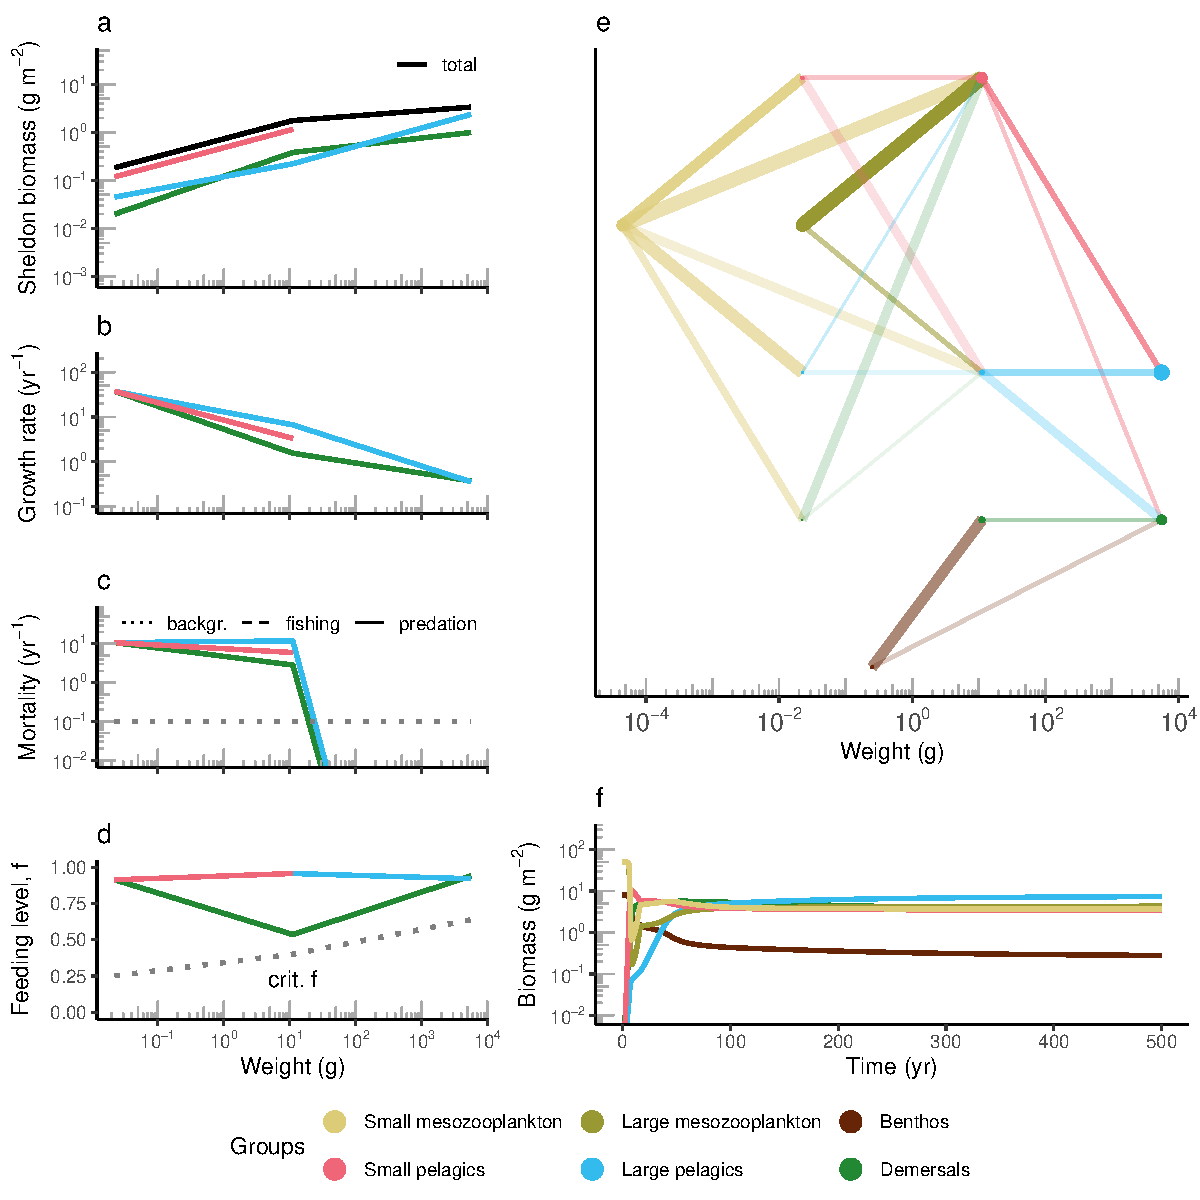
\includegraphics{C:/Users/Admin/Desktop/pkg-oct/FEISTY/vignettes/FEISTY_files/figure-latex/unnamed-chunk-3-1.pdf}

This figure collection includes \texttt{plotSpectra()},
\texttt{plotRates()}, \texttt{plotNetwork()}, and
\texttt{plotBiomasstime()}. Each of these can be called independently.
For instance:

\begin{Shaded}
\begin{Highlighting}[]
\FunctionTok{plotBiomasstime}\NormalTok{(sim)}
\end{Highlighting}
\end{Shaded}

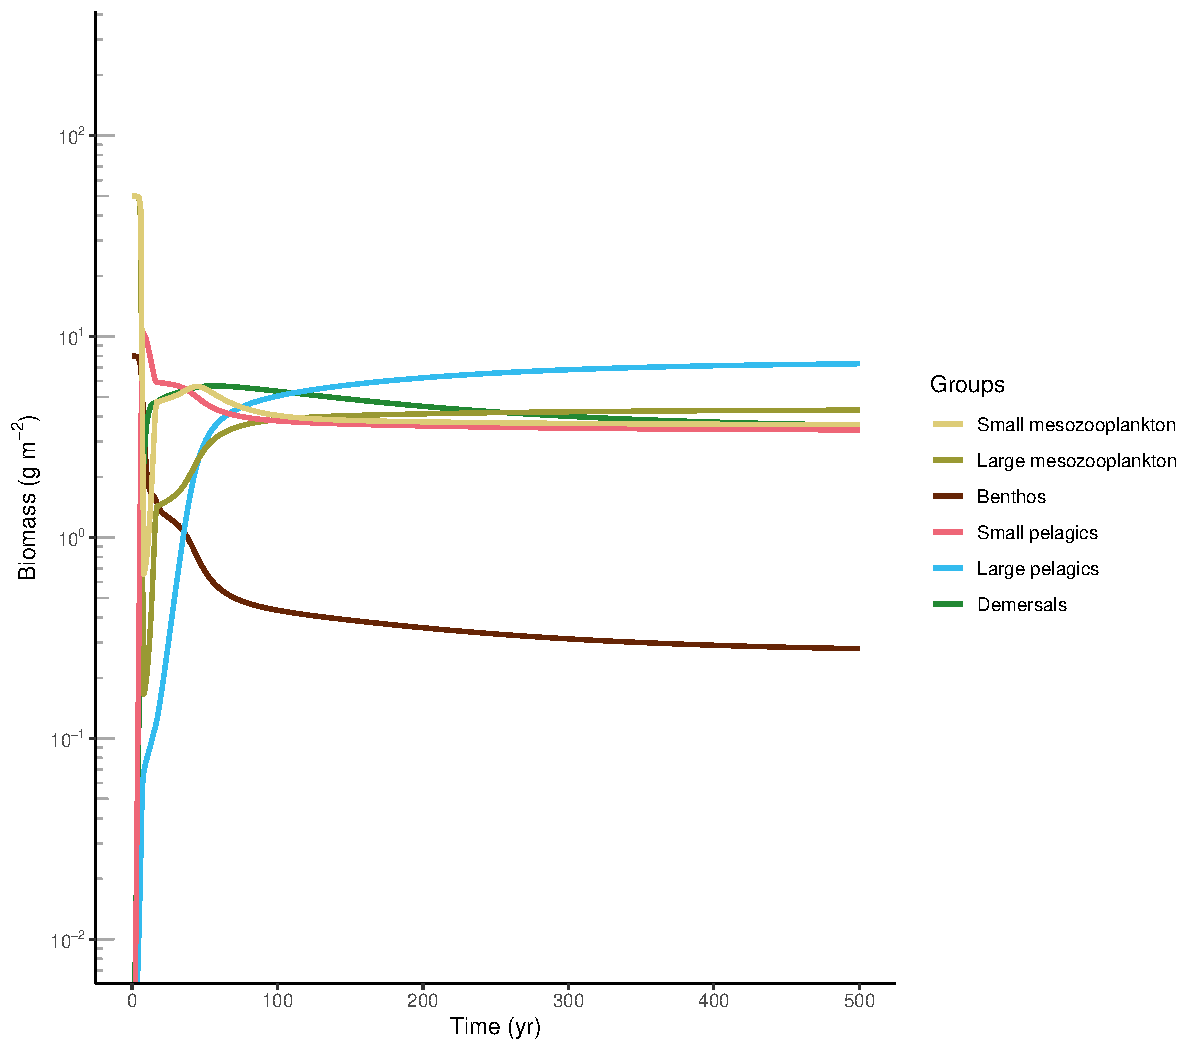
\includegraphics{C:/Users/Admin/Desktop/pkg-oct/FEISTY/vignettes/FEISTY_files/figure-latex/unnamed-chunk-4-1.pdf}

\begin{Shaded}
\begin{Highlighting}[]
\FunctionTok{plotRates}\NormalTok{(sim)}
\end{Highlighting}
\end{Shaded}

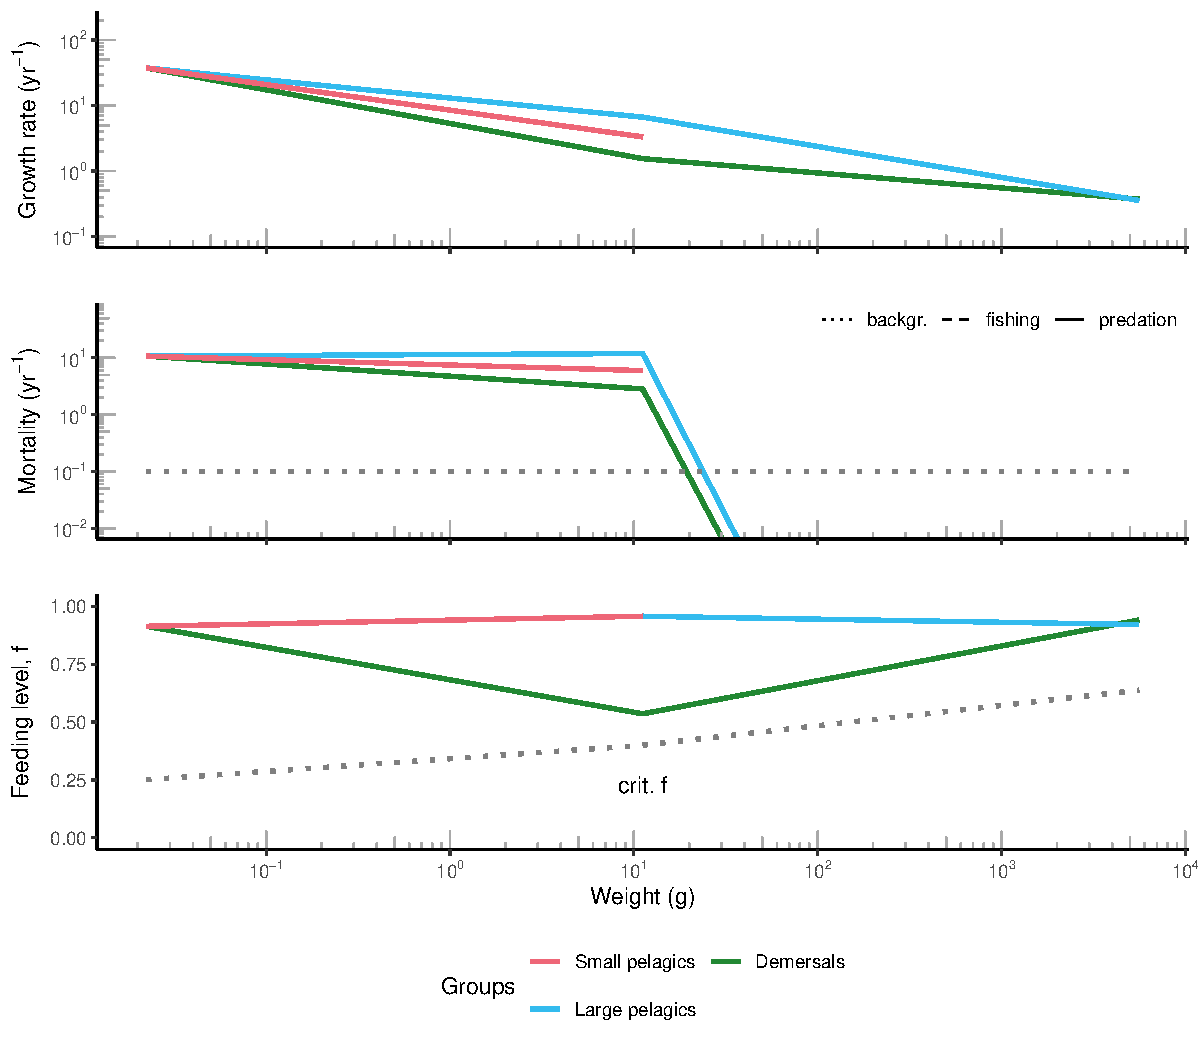
\includegraphics{C:/Users/Admin/Desktop/pkg-oct/FEISTY/vignettes/FEISTY_files/figure-latex/unnamed-chunk-5-1.pdf}

\hypertarget{fishing-mortality-assignment}{%
\subsection{Fishing mortality
assignment}\label{fishing-mortality-assignment}}

For simplicity, arguments of fishing in \texttt{setupbasic()} and
\texttt{setupVertical()} only allow assigning fishing mortality to all
functional types. Although the parameter set has been generated by
calling setup functions e.g., \texttt{setupVertical()}, it is feasible
to overwrite parameters manually. As a result, fishing mortality for a
specific functional type can be assigned afterwards.

\begin{Shaded}
\begin{Highlighting}[]
\NormalTok{p}\OtherTok{=}\FunctionTok{setupVertical2}\NormalTok{(}\AttributeTok{szprod=} \DecValTok{120}\NormalTok{,}
                 \AttributeTok{lzprod =} \DecValTok{120}\NormalTok{,}
                 \AttributeTok{dfpho=}\DecValTok{200}\NormalTok{, }
                 \AttributeTok{depth =} \DecValTok{700}\NormalTok{, }
                 \AttributeTok{nStages =} \DecValTok{9}\NormalTok{, }
                 \AttributeTok{F=}\DecValTok{0}\NormalTok{) }\CommentTok{\# no fishing for all size classes}
\FunctionTok{names}\NormalTok{(p}\SpecialCharTok{$}\NormalTok{mortF)}\OtherTok{=}\NormalTok{p}\SpecialCharTok{$}\NormalTok{stagenames}
\NormalTok{df}\OtherTok{=}\FunctionTok{data.frame}\NormalTok{(}\AttributeTok{mortF\_original=}\FunctionTok{c}\NormalTok{(p}\SpecialCharTok{$}\NormalTok{mortF[p}\SpecialCharTok{$}\NormalTok{ix[[}\DecValTok{1}\NormalTok{]]],p}\SpecialCharTok{$}\NormalTok{mortF[p}\SpecialCharTok{$}\NormalTok{ix[[}\DecValTok{5}\NormalTok{]]]))}
\CommentTok{\# assign 0.2/year as the maximum fishing mortality to small pelagic fish}
\NormalTok{p}\OtherTok{=}\FunctionTok{setFishing}\NormalTok{(}\AttributeTok{p=}\NormalTok{p,}\AttributeTok{F=}\FloatTok{0.2}\NormalTok{,}\AttributeTok{etaF=}\FloatTok{0.05}\NormalTok{,}\AttributeTok{groupidx=}\FunctionTok{c}\NormalTok{(}\DecValTok{1}\NormalTok{))}
\CommentTok{\# assign 0.3/year as the maximum fishing mortality to demersal fish}
\NormalTok{p}\OtherTok{=}\FunctionTok{setFishing}\NormalTok{(}\AttributeTok{p=}\NormalTok{p,}\AttributeTok{F=}\FloatTok{0.3}\NormalTok{,}\AttributeTok{etaF=}\FloatTok{0.05}\NormalTok{,}\AttributeTok{groupidx=}\FunctionTok{c}\NormalTok{(}\DecValTok{5}\NormalTok{))}
\NormalTok{df}\OtherTok{=}\FunctionTok{cbind}\NormalTok{(df,}\FunctionTok{data.frame}\NormalTok{(}\AttributeTok{mortF\_new=}\FunctionTok{c}\NormalTok{(p}\SpecialCharTok{$}\NormalTok{mortF[p}\SpecialCharTok{$}\NormalTok{ix[[}\DecValTok{1}\NormalTok{]]],p}\SpecialCharTok{$}\NormalTok{mortF[p}\SpecialCharTok{$}\NormalTok{ix[[}\DecValTok{5}\NormalTok{]]])))}
\NormalTok{knitr}\SpecialCharTok{::}\FunctionTok{kable}\NormalTok{(df,}\AttributeTok{caption=}\StringTok{"Fishing mortality before and after assignment"}\NormalTok{)}
\end{Highlighting}
\end{Shaded}

\begin{longtable}[]{@{}lrr@{}}
\caption{Fishing mortality before and after assignment}\tabularnewline
\toprule()
& mortF\_original & mortF\_new \\
\midrule()
\endfirsthead
\toprule()
& mortF\_original & mortF\_new \\
\midrule()
\endhead
smallPel\_1 & 0 & 0.0000000 \\
smallPel\_2 & 0 & 0.0000000 \\
smallPel\_3 & 0 & 0.0000006 \\
smallPel\_4 & 0 & 0.0002858 \\
smallPel\_5 & 0 & 0.0834188 \\
smallPel\_6 & 0 & 0.1994425 \\
demersals\_1 & 0 & 0.0000000 \\
demersals\_2 & 0 & 0.0000000 \\
demersals\_3 & 0 & 0.0000000 \\
demersals\_4 & 0 & 0.0000000 \\
demersals\_5 & 0 & 0.0000000 \\
demersals\_6 & 0 & 0.0000009 \\
demersals\_7 & 0 & 0.0004287 \\
demersals\_8 & 0 & 0.1251281 \\
demersals\_9 & 0 & 0.2991638 \\
\bottomrule()
\end{longtable}

\begin{Shaded}
\begin{Highlighting}[]
\NormalTok{df}\OtherTok{=}\FunctionTok{data.frame}\NormalTok{(}\StringTok{"Stage"}\OtherTok{=}\DecValTok{1}\SpecialCharTok{:}\FunctionTok{length}\NormalTok{(p}\SpecialCharTok{$}\NormalTok{ix[[}\DecValTok{1}\NormalTok{]]), }\StringTok{"mortF"}\OtherTok{=}\NormalTok{p}\SpecialCharTok{$}\NormalTok{mortF[p}\SpecialCharTok{$}\NormalTok{ix[[}\DecValTok{1}\NormalTok{]]],}\StringTok{"Groups"}\OtherTok{=}\StringTok{"smallPel"}\NormalTok{)}
\NormalTok{df}\OtherTok{=}\FunctionTok{rbind}\NormalTok{(df,}\FunctionTok{data.frame}\NormalTok{(}\StringTok{"Stage"}\OtherTok{=}\DecValTok{1}\SpecialCharTok{:}\FunctionTok{length}\NormalTok{(p}\SpecialCharTok{$}\NormalTok{ix[[}\DecValTok{5}\NormalTok{]]), }
                       \StringTok{"mortF"}\OtherTok{=}\NormalTok{p}\SpecialCharTok{$}\NormalTok{mortF[p}\SpecialCharTok{$}\NormalTok{ix[[}\DecValTok{5}\NormalTok{]]],}\StringTok{"Groups"}\OtherTok{=}\StringTok{"demersals"}\NormalTok{))}
\NormalTok{df}\SpecialCharTok{$}\NormalTok{Groups}\OtherTok{=}\FunctionTok{factor}\NormalTok{(df}\SpecialCharTok{$}\NormalTok{Groups,}\AttributeTok{levels=}\FunctionTok{c}\NormalTok{(}\StringTok{"smallPel"}\NormalTok{,}\StringTok{"demersals"}\NormalTok{))}
\CommentTok{\# plot of fishing mortality of small pelagics and demersals}
\NormalTok{fig}\OtherTok{=}\FunctionTok{ggplot}\NormalTok{(df, }\FunctionTok{aes}\NormalTok{(}\AttributeTok{x =}\NormalTok{ Stage, }\AttributeTok{y =}\NormalTok{ mortF, }\AttributeTok{color =}\NormalTok{ Groups))}\SpecialCharTok{+}
    \FunctionTok{geom\_line}\NormalTok{(}\AttributeTok{linewidth =} \FloatTok{0.7}\NormalTok{,}\AttributeTok{alpha=}\FloatTok{0.9}\NormalTok{)}\SpecialCharTok{+}
    \FunctionTok{geom\_point}\NormalTok{(}\AttributeTok{size=}\FloatTok{1.5}\NormalTok{,}\AttributeTok{alpha=}\FloatTok{0.9}\NormalTok{)}\SpecialCharTok{+}
  \FunctionTok{labs}\NormalTok{(}\AttributeTok{x =} \FunctionTok{expression}\NormalTok{(}\StringTok{"Stage"}\NormalTok{), }\AttributeTok{y =} \FunctionTok{expression}\NormalTok{(}\StringTok{"Fishing mortality"}\SpecialCharTok{\textasciitilde{}}\NormalTok{(yr}\SpecialCharTok{\^{}}\NormalTok{\{}\SpecialCharTok{{-}}\DecValTok{1}\NormalTok{\}))) }\SpecialCharTok{+}
  \FunctionTok{scale\_color\_manual}\NormalTok{(}\AttributeTok{values =} \FunctionTok{c}\NormalTok{(}\StringTok{"red"}\NormalTok{, }\StringTok{"black"}\NormalTok{),}\AttributeTok{labels=}\FunctionTok{c}\NormalTok{(}\StringTok{"Small pelagics"}\NormalTok{,}\StringTok{"Demersals"}\NormalTok{)) }\SpecialCharTok{+}
  \FunctionTok{scale\_x\_continuous}\NormalTok{(}\AttributeTok{breaks =} \FunctionTok{unique}\NormalTok{(df}\SpecialCharTok{$}\NormalTok{Stage))}\SpecialCharTok{+}
      \FunctionTok{theme}\NormalTok{(}\AttributeTok{panel.background =} \FunctionTok{element\_rect}\NormalTok{(}\AttributeTok{fill =} \StringTok{"white"}\NormalTok{),}
          \AttributeTok{panel.border =} \FunctionTok{element\_rect}\NormalTok{(}\AttributeTok{color =} \StringTok{"black"}\NormalTok{, }\AttributeTok{fill =} \ConstantTok{NA}\NormalTok{),}
          \AttributeTok{axis.line =} \FunctionTok{element\_line}\NormalTok{(}\AttributeTok{color =} \StringTok{"black"}\NormalTok{),}
          \CommentTok{\#legend.title = element\_blank(),}
          \AttributeTok{legend.key =} \FunctionTok{element\_rect}\NormalTok{(}\AttributeTok{fill =} \StringTok{"transparent"}\NormalTok{, }\AttributeTok{color =} \StringTok{"transparent"}\NormalTok{),}
          \AttributeTok{legend.position =} \StringTok{"bottom"}\NormalTok{)}
  
\NormalTok{fig}
\end{Highlighting}
\end{Shaded}

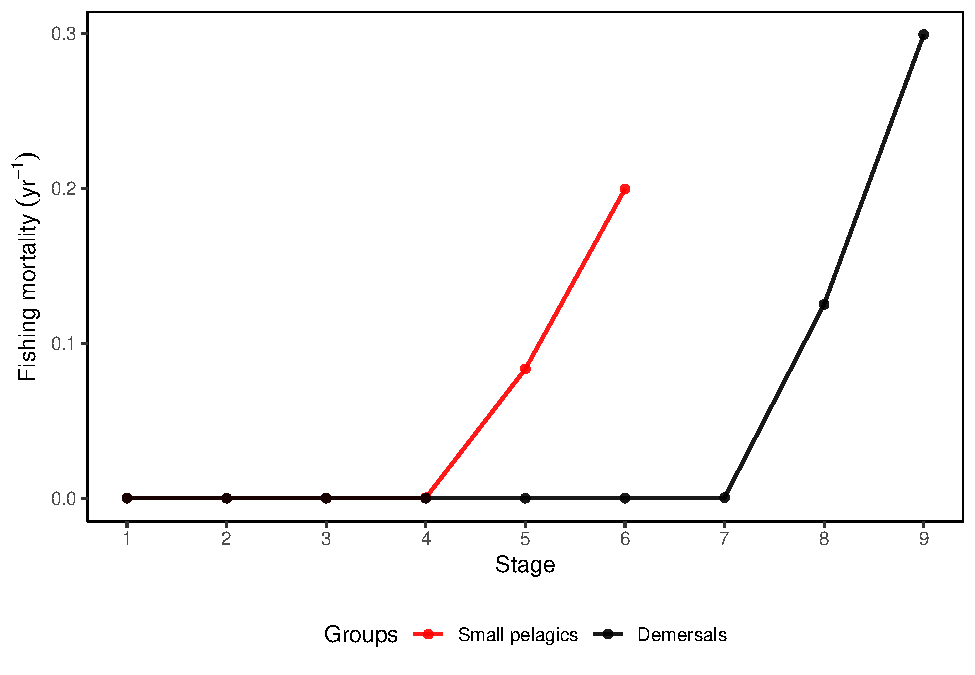
\includegraphics{C:/Users/Admin/Desktop/pkg-oct/FEISTY/vignettes/FEISTY_files/figure-latex/unnamed-chunk-6-1.pdf}

Since fishing mortality was assigned manually to two of three fish
functional types, which is not the ready-to-use function
\texttt{setupXXX()} can do, we must turn on \texttt{USEdll} and
\texttt{bCust} flags for simulations. It means we want to run the
simulation based on a parameter set we customized. All core parameters
for simulation will be transmitted from R to Fortran dll rather than
generated in Fortran. These two flags are TRUE as default. If
\texttt{USEdll\ =\ F}, it means the simulation is done in R (slower but
helpful when debugging).

\begin{Shaded}
\begin{Highlighting}[]
\NormalTok{sim}\OtherTok{=}\FunctionTok{simulateFEISTY}\NormalTok{(}\AttributeTok{p =}\NormalTok{ p, }\AttributeTok{tEnd =} \DecValTok{200}\NormalTok{, }\AttributeTok{USEdll =}\NormalTok{ T, }\AttributeTok{bCust =}\NormalTok{ T)}
\end{Highlighting}
\end{Shaded}

The following functions can be used for visualizing yield and spawning
stock biomass changes over time.

\begin{Shaded}
\begin{Highlighting}[]
\FunctionTok{plotYieldtime}\NormalTok{(sim)}
\end{Highlighting}
\end{Shaded}

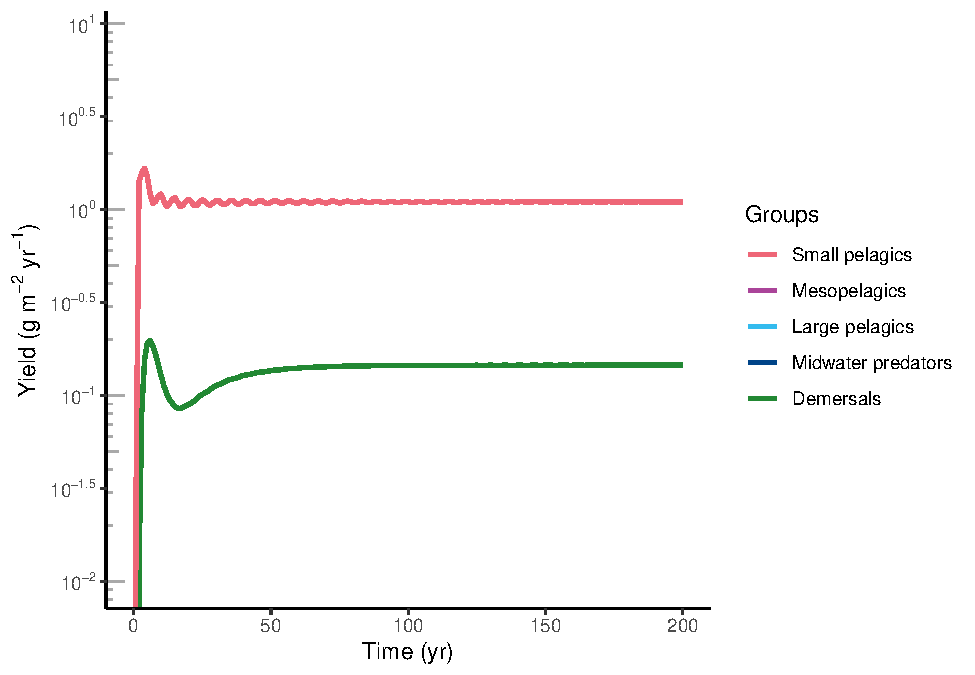
\includegraphics{C:/Users/Admin/Desktop/pkg-oct/FEISTY/vignettes/FEISTY_files/figure-latex/unnamed-chunk-8-1.pdf}

\begin{Shaded}
\begin{Highlighting}[]
\FunctionTok{plotSSBtime}\NormalTok{(sim)}
\end{Highlighting}
\end{Shaded}

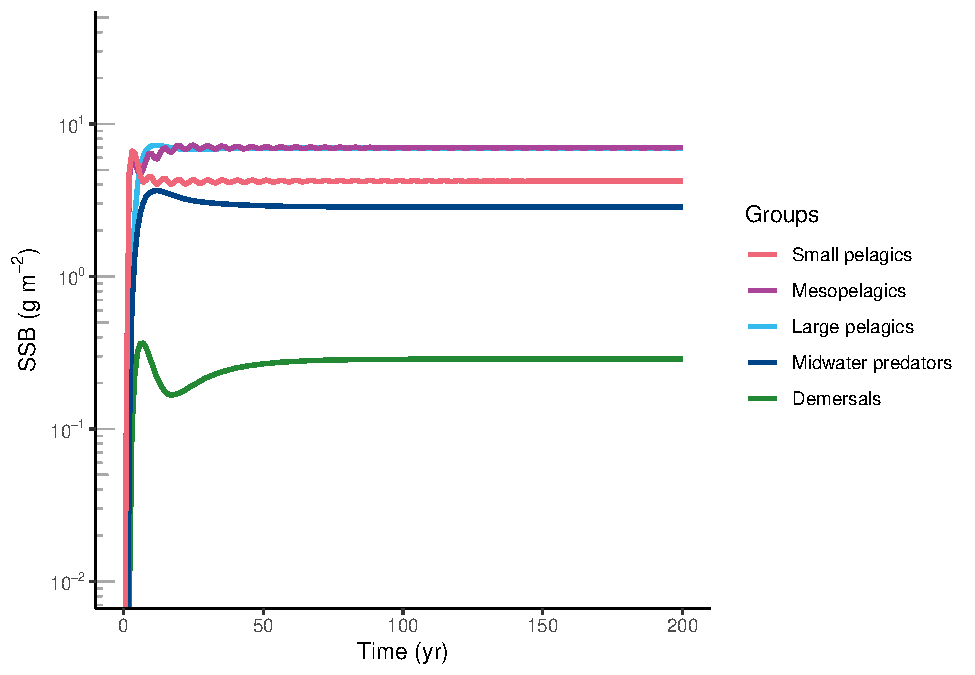
\includegraphics{C:/Users/Admin/Desktop/pkg-oct/FEISTY/vignettes/FEISTY_files/figure-latex/unnamed-chunk-9-1.pdf}

\hypertarget{bottom-up-control-examples}{%
\subsection{Bottom-up control
examples}\label{bottom-up-control-examples}}

One of the goals of the FEISTY model is to obtain emergent fish food
webs that vary with environmental conditions (i.e.~bottom-up mechanisms
that control fish communities). Here we demonstrate two model runs with
one describing an oligotrophic system and the other one a more eutrophic
system based on \texttt{setupVertical2}.

\begin{Shaded}
\begin{Highlighting}[]
\NormalTok{p1}\OtherTok{=}\FunctionTok{setupVertical2}\NormalTok{(}\AttributeTok{depth=}\DecValTok{1000}\NormalTok{,}\AttributeTok{szprod=}\DecValTok{5}\NormalTok{, }\AttributeTok{lzprod=}\DecValTok{5}\NormalTok{,}\AttributeTok{dfpho =} \DecValTok{130}\NormalTok{) }\CommentTok{\# oligotrophic 1000 meter}
\NormalTok{p2}\OtherTok{=}\FunctionTok{setupVertical2}\NormalTok{(}\AttributeTok{depth=}\DecValTok{1000}\NormalTok{,}\AttributeTok{szprod=}\DecValTok{100}\NormalTok{, }\AttributeTok{lzprod=}\DecValTok{100}\NormalTok{,}\AttributeTok{dfpho =}\DecValTok{380}\NormalTok{) }\CommentTok{\# eutrophic 1000 meter}
\end{Highlighting}
\end{Shaded}

In the oligotrophic water, large pelagic fish, midwater predators, and
demersal fish cannot survive (panel f), since the resource productions
are low and do not provide enough food for them (panel d).

\begin{Shaded}
\begin{Highlighting}[]
\NormalTok{sim1}\OtherTok{=}\FunctionTok{simulateFEISTY}\NormalTok{(}\AttributeTok{p=}\NormalTok{p1,}\AttributeTok{tEnd=}\DecValTok{500}\NormalTok{)}
\FunctionTok{plotSimulation}\NormalTok{(sim1)}
\end{Highlighting}
\end{Shaded}

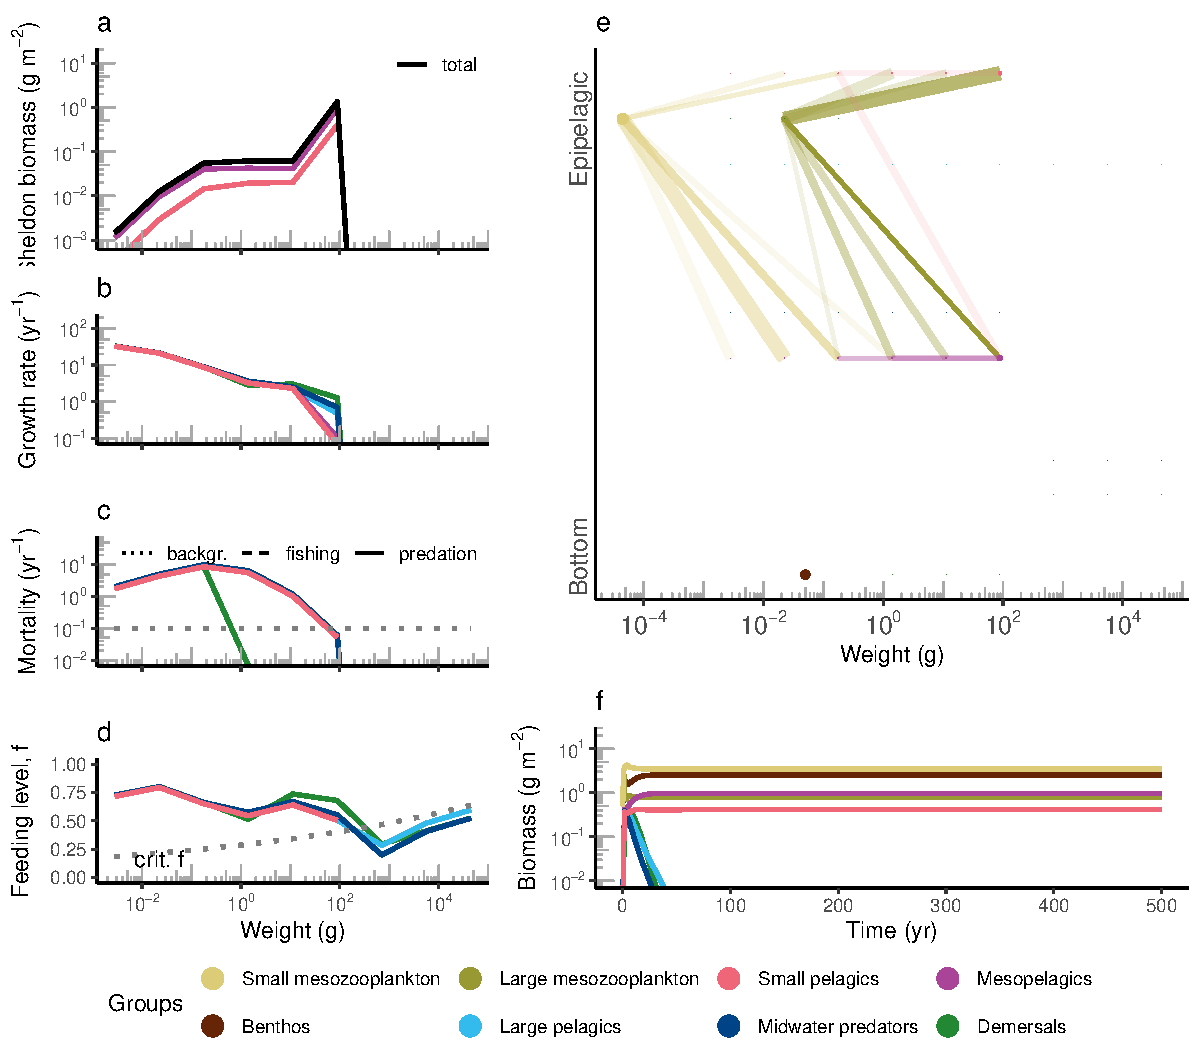
\includegraphics{C:/Users/Admin/Desktop/pkg-oct/FEISTY/vignettes/FEISTY_files/figure-latex/unnamed-chunk-11-1.pdf}

On the contrary, in the eutrophic water, high resource productions
support the existence of all five functional types (panel f). All fish
have feeding levels that are higher than their critical feeding levels
(panel d).

\begin{Shaded}
\begin{Highlighting}[]
\NormalTok{sim2}\OtherTok{=}\FunctionTok{simulateFEISTY}\NormalTok{(}\AttributeTok{p=}\NormalTok{p2,}\AttributeTok{tEnd=}\DecValTok{500}\NormalTok{)}
\FunctionTok{plotSimulation}\NormalTok{(sim2)}
\end{Highlighting}
\end{Shaded}

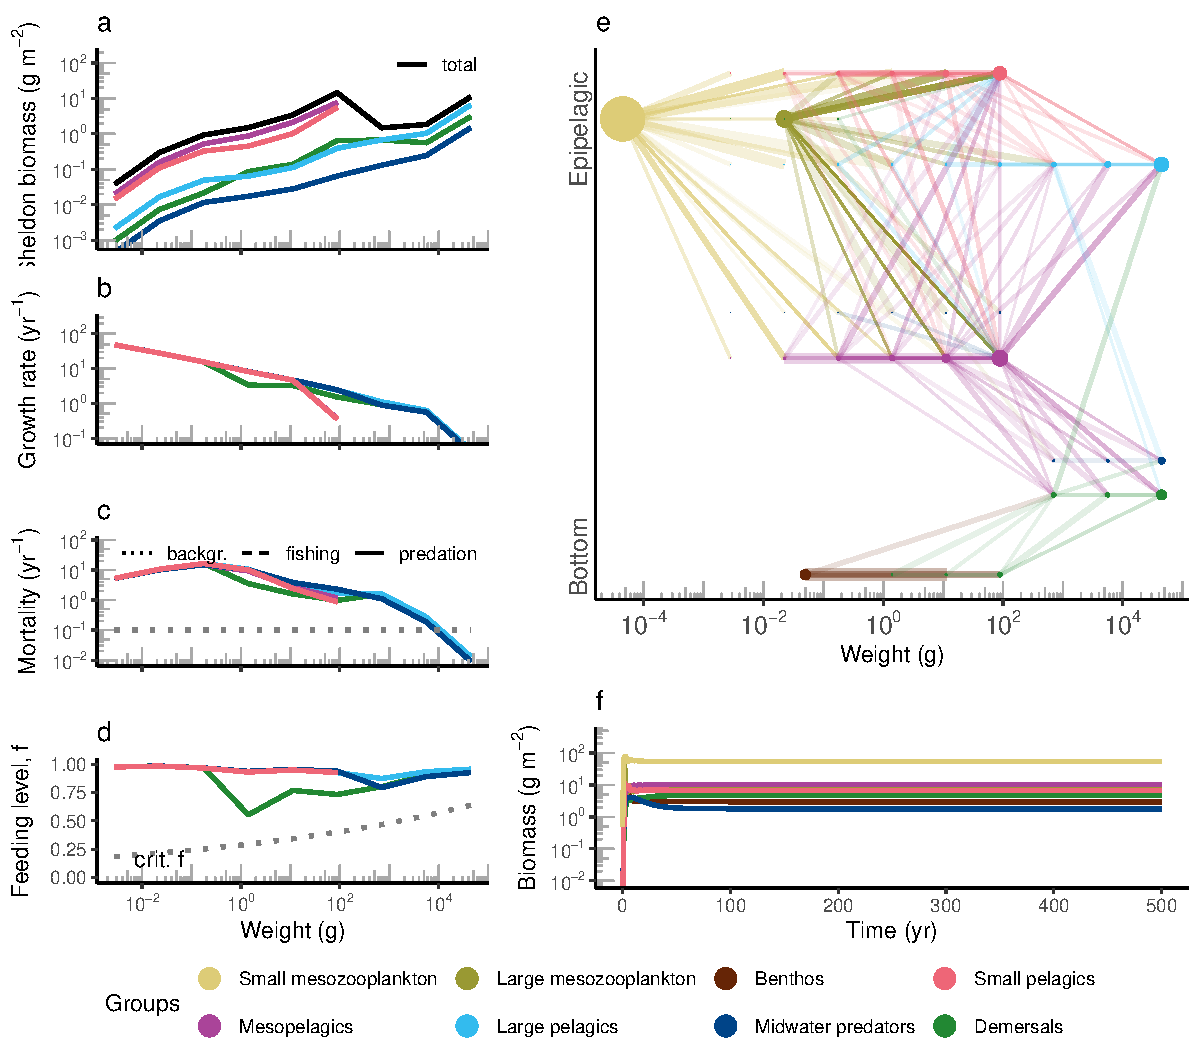
\includegraphics{C:/Users/Admin/Desktop/pkg-oct/FEISTY/vignettes/FEISTY_files/figure-latex/unnamed-chunk-12-1.pdf}

\newpage

\hypertarget{references}{%
\section{References}\label{references}}

\bibliography{references.bib}

\hypertarget{refs}{}
\begin{CSLReferences}{1}{0}
\leavevmode\vadjust pre{\hypertarget{ref-andersen2019fish}{}}%
Andersen, Ken H. 2019. \emph{Fish Ecology, Evolution, and Exploitation:
A New Theoretical Synthesis}. Princeton University Press.

\leavevmode\vadjust pre{\hypertarget{ref-deRoos2008}{}}%
De Roos, André M, Tim Schellekens, Tobias Van Kooten, Karen Van De
Wolfshaar, David Claessen, and Lennart Persson. 2008. {``Simplifying a
Physiologically Structured Population Model to a Stage-Structured
Biomass Model.''} \emph{Theoretical Population Biology} 73 (1): 47--62.

\leavevmode\vadjust pre{\hypertarget{ref-van2021emergent}{}}%
Denderen, P Daniël van, Colleen M Petrik, Charles A Stock, and Ken H
Andersen. 2021. {``Emergent Global Biogeography of Marine Fish Food
Webs.''} \emph{Global Ecology and Biogeography} 30 (9): 1822--34.

\leavevmode\vadjust pre{\hypertarget{ref-petrik2019bottom}{}}%
Petrik, Colleen M, Charles A Stock, Ken H Andersen, P Daniël van
Denderen, and James R Watson. 2019. {``Bottom-up Drivers of Global
Patterns of Demersal, Forage, and Pelagic Fishes.''} \emph{Progress in
Oceanography} 176: 102124.

\end{CSLReferences}

\end{document}
